\documentclass[12pt,a4paper]{article}

% ── Packages ──
\usepackage[utf8]{inputenc}
\usepackage[T1]{fontenc}
\usepackage{lmodern}
\usepackage[margin=0.85in]{geometry}
\usepackage{graphicx}
\usepackage{xcolor}
\usepackage{hyperref}
\usepackage{fancyhdr}
\usepackage{enumitem}
\usepackage{booktabs}
\usepackage{float}
\usepackage{caption}
\usepackage{parskip}
\usepackage{setspace}
\usepackage{tcolorbox}
\usepackage{fancybox}

% ── Colors ──
\definecolor{blue}{HTML}{2563EB}
\definecolor{dark}{HTML}{0A0E1A}
\definecolor{gray}{HTML}{3A3F52}
\definecolor{lightgray}{HTML}{8B92A8}
\definecolor{lightbg}{HTML}{F7F8FC}

% ── Page Border ──
\usepackage{eso-pic}
\usepackage{atbegshi}

\newcommand{\pageborder}{%
  \AtBeginShipout{%
    \AtBeginShipoutUpperLeft{%
      \put(\dimexpr 1in-\fboxsep-0.6pt\relax,%
           \dimexpr -1in+\fboxsep+0.6pt\relax){%
        \raisebox{-\height}{%
          \rule{0pt}{\dimexpr \paperheight-2in+2\fboxsep+1.2pt\relax}%
          \rule{0pt}{0pt}%
          \color{blue!40}\fboxsep=0pt\fboxrule=1.2pt%
          \framebox[\dimexpr \paperwidth-2in+2\fboxsep+1.2pt\relax]{%
            \rule[-\dimexpr \paperheight-2in+2\fboxsep\relax]{0pt}{%
              \dimexpr \paperheight-2in+2\fboxsep\relax}%
          }%
        }%
      }%
    }%
  }%
}

% Simpler page border using background
\AddToShipoutPictureBG{%
  \AtPageLowerLeft{%
    \put(\LenToUnit{0.6in},\LenToUnit{0.6in}){%
      \color{blue!35}%
      \framebox(\LenToUnit{\dimexpr\paperwidth-1.2in},\LenToUnit{\dimexpr\paperheight-1.2in}){}%
    }%
  }%
}

% ── Hyperref ──
\hypersetup{
  colorlinks=true,
  linkcolor=blue,
  urlcolor=blue,
  pdftitle={Basic Prompt Writing - B25ETC23 Report},
}

% ── Headers/Footers ──
\pagestyle{fancy}
\fancyhf{}
\fancyhead[L]{\small\textcolor{lightgray}{B25ETC23 -- Introduction to AI}}
\fancyhead[R]{\small\textcolor{lightgray}{Basic Prompt Writing}}
\fancyfoot[C]{\small\thepage}
\renewcommand{\headrulewidth}{0.4pt}

% ── Caption styling ──
\captionsetup{font=small, labelfont={bf,color=blue}, labelsep=pipe}

% ── Image path ──
\graphicspath{{slides/}}

% ── Spacing ──
\onehalfspacing

\begin{document}

% ════════════════════════════════════════════
%  TABLE OF CONTENTS
% ════════════════════════════════════════════
\begin{center}
{\LARGE\bfseries\textcolor{dark}{Table of Contents}}\\[0.3cm]
\rule{0.4\textwidth}{0.8pt}
\end{center}

\vspace{0.8cm}

\begin{center}
\begin{minipage}{0.85\textwidth}
\noindent\textbf{\textcolor{blue}{Abstract}} \dotfill \pageref{sec:abstract}

\vspace{0.6cm}
\noindent\textbf{\textcolor{blue}{Slide Deck Presentation}}\\[0.2cm]
\hspace{0.5cm}Slide 1 -- Title Slide \dotfill \pageref{sec:s1}\\[0.15cm]
\hspace{0.5cm}Slide 2 -- What is Prompt Engineering? \dotfill \pageref{sec:s2}\\[0.15cm]
\hspace{0.5cm}Slide 3 -- Why Prompts Matter \dotfill \pageref{sec:s3}\\[0.15cm]
\hspace{0.5cm}Slide 4 -- The Electricity Experiment \dotfill \pageref{sec:s4}\\[0.15cm]
\hspace{0.5cm}Slide 5 -- The Vague Prompt Response \dotfill \pageref{sec:s5}\\[0.15cm]
\hspace{0.5cm}Slide 6 -- The Specific Prompt Response \dotfill \pageref{sec:s6}\\[0.15cm]
\hspace{0.5cm}Slide 7 -- Side-by-Side Comparison \dotfill \pageref{sec:s7}\\[0.15cm]
\hspace{0.5cm}Slide 8 -- Why the Specific Prompt Succeeded \dotfill \pageref{sec:s8}\\[0.15cm]
\hspace{0.5cm}Slide 9 -- The CATO Framework \dotfill \pageref{sec:s9}\\[0.15cm]
\hspace{0.5cm}Slide 10 -- Tips and Best Practices \dotfill \pageref{sec:s10}\\[0.15cm]
\hspace{0.5cm}Slide 11 -- Real-World Applications \dotfill \pageref{sec:s11}\\[0.15cm]
\hspace{0.5cm}Slide 12 -- Conclusion \dotfill \pageref{sec:s12}
\end{minipage}
\end{center}

\newpage

% ════════════════════════════════════════════
%  ABSTRACT
% ════════════════════════════════════════════
\label{sec:abstract}
\begin{center}
{\LARGE\bfseries\textcolor{dark}{Abstract}}\\[0.3cm]
\rule{0.4\textwidth}{0.8pt}
\end{center}

\vspace{0.5cm}

This report documents a presentation on \textbf{Basic Prompt Writing} delivered as part of the B25ETC23 Introduction to AI course. The presentation investigates a fundamental question in human-AI interaction: \emph{does the way you phrase a question to an AI actually matter?}

To answer this, we designed a controlled experiment using \textbf{Electricity} as the test topic. Two prompts were crafted -- one vague (\emph{``Tell me about electricity.''}) and one specific (\emph{``Explain how electricity is generated in a thermal power plant and how it reaches homes through the power grid, in simple terms for a high school student.''}) -- and fed to the same AI model (ChatGPT). The results were analysed across four quality dimensions: Usefulness, Clarity, Relevance, and Actionability.

The specific prompt outperformed the vague prompt by a factor of \textbf{3.4x} across all quality metrics, demonstrating that prompt construction is the single most influential variable in determining AI output quality. From this experiment, we derived a practical four-part framework -- the \textbf{CATO Formula} (Context, Action, Target Audience, Output Format) -- as a repeatable methodology for writing effective prompts.

This report includes the full slide deck with annotated commentary covering the theoretical foundation, the experiment, comparative analysis, the CATO framework, practical tips, and real-world applications of prompt engineering.

\vspace{0.5cm}
\noindent\textbf{Keywords:} Prompt Engineering, AI Interaction, Large Language Models, CATO Framework, ChatGPT, Human-AI Collaboration

\newpage

% ════════════════════════════════════════════
%  SLIDE DECK PRESENTATION
% ════════════════════════════════════════════
\begin{center}
{\LARGE\bfseries\textcolor{dark}{Slide Deck Presentation}}\\[0.3cm]
\rule{0.4\textwidth}{0.8pt}
\end{center}

\vspace{0.3cm}

This section presents all 12 slides from the presentation with accompanying commentary. Slides were captured from the live HTML presentation using Playwright automated screenshots.

% ── Slide 1 ──
\subsection*{Slide 1 -- Title Slide}
\label{sec:s1}

\begin{figure}[H]
  \centering
  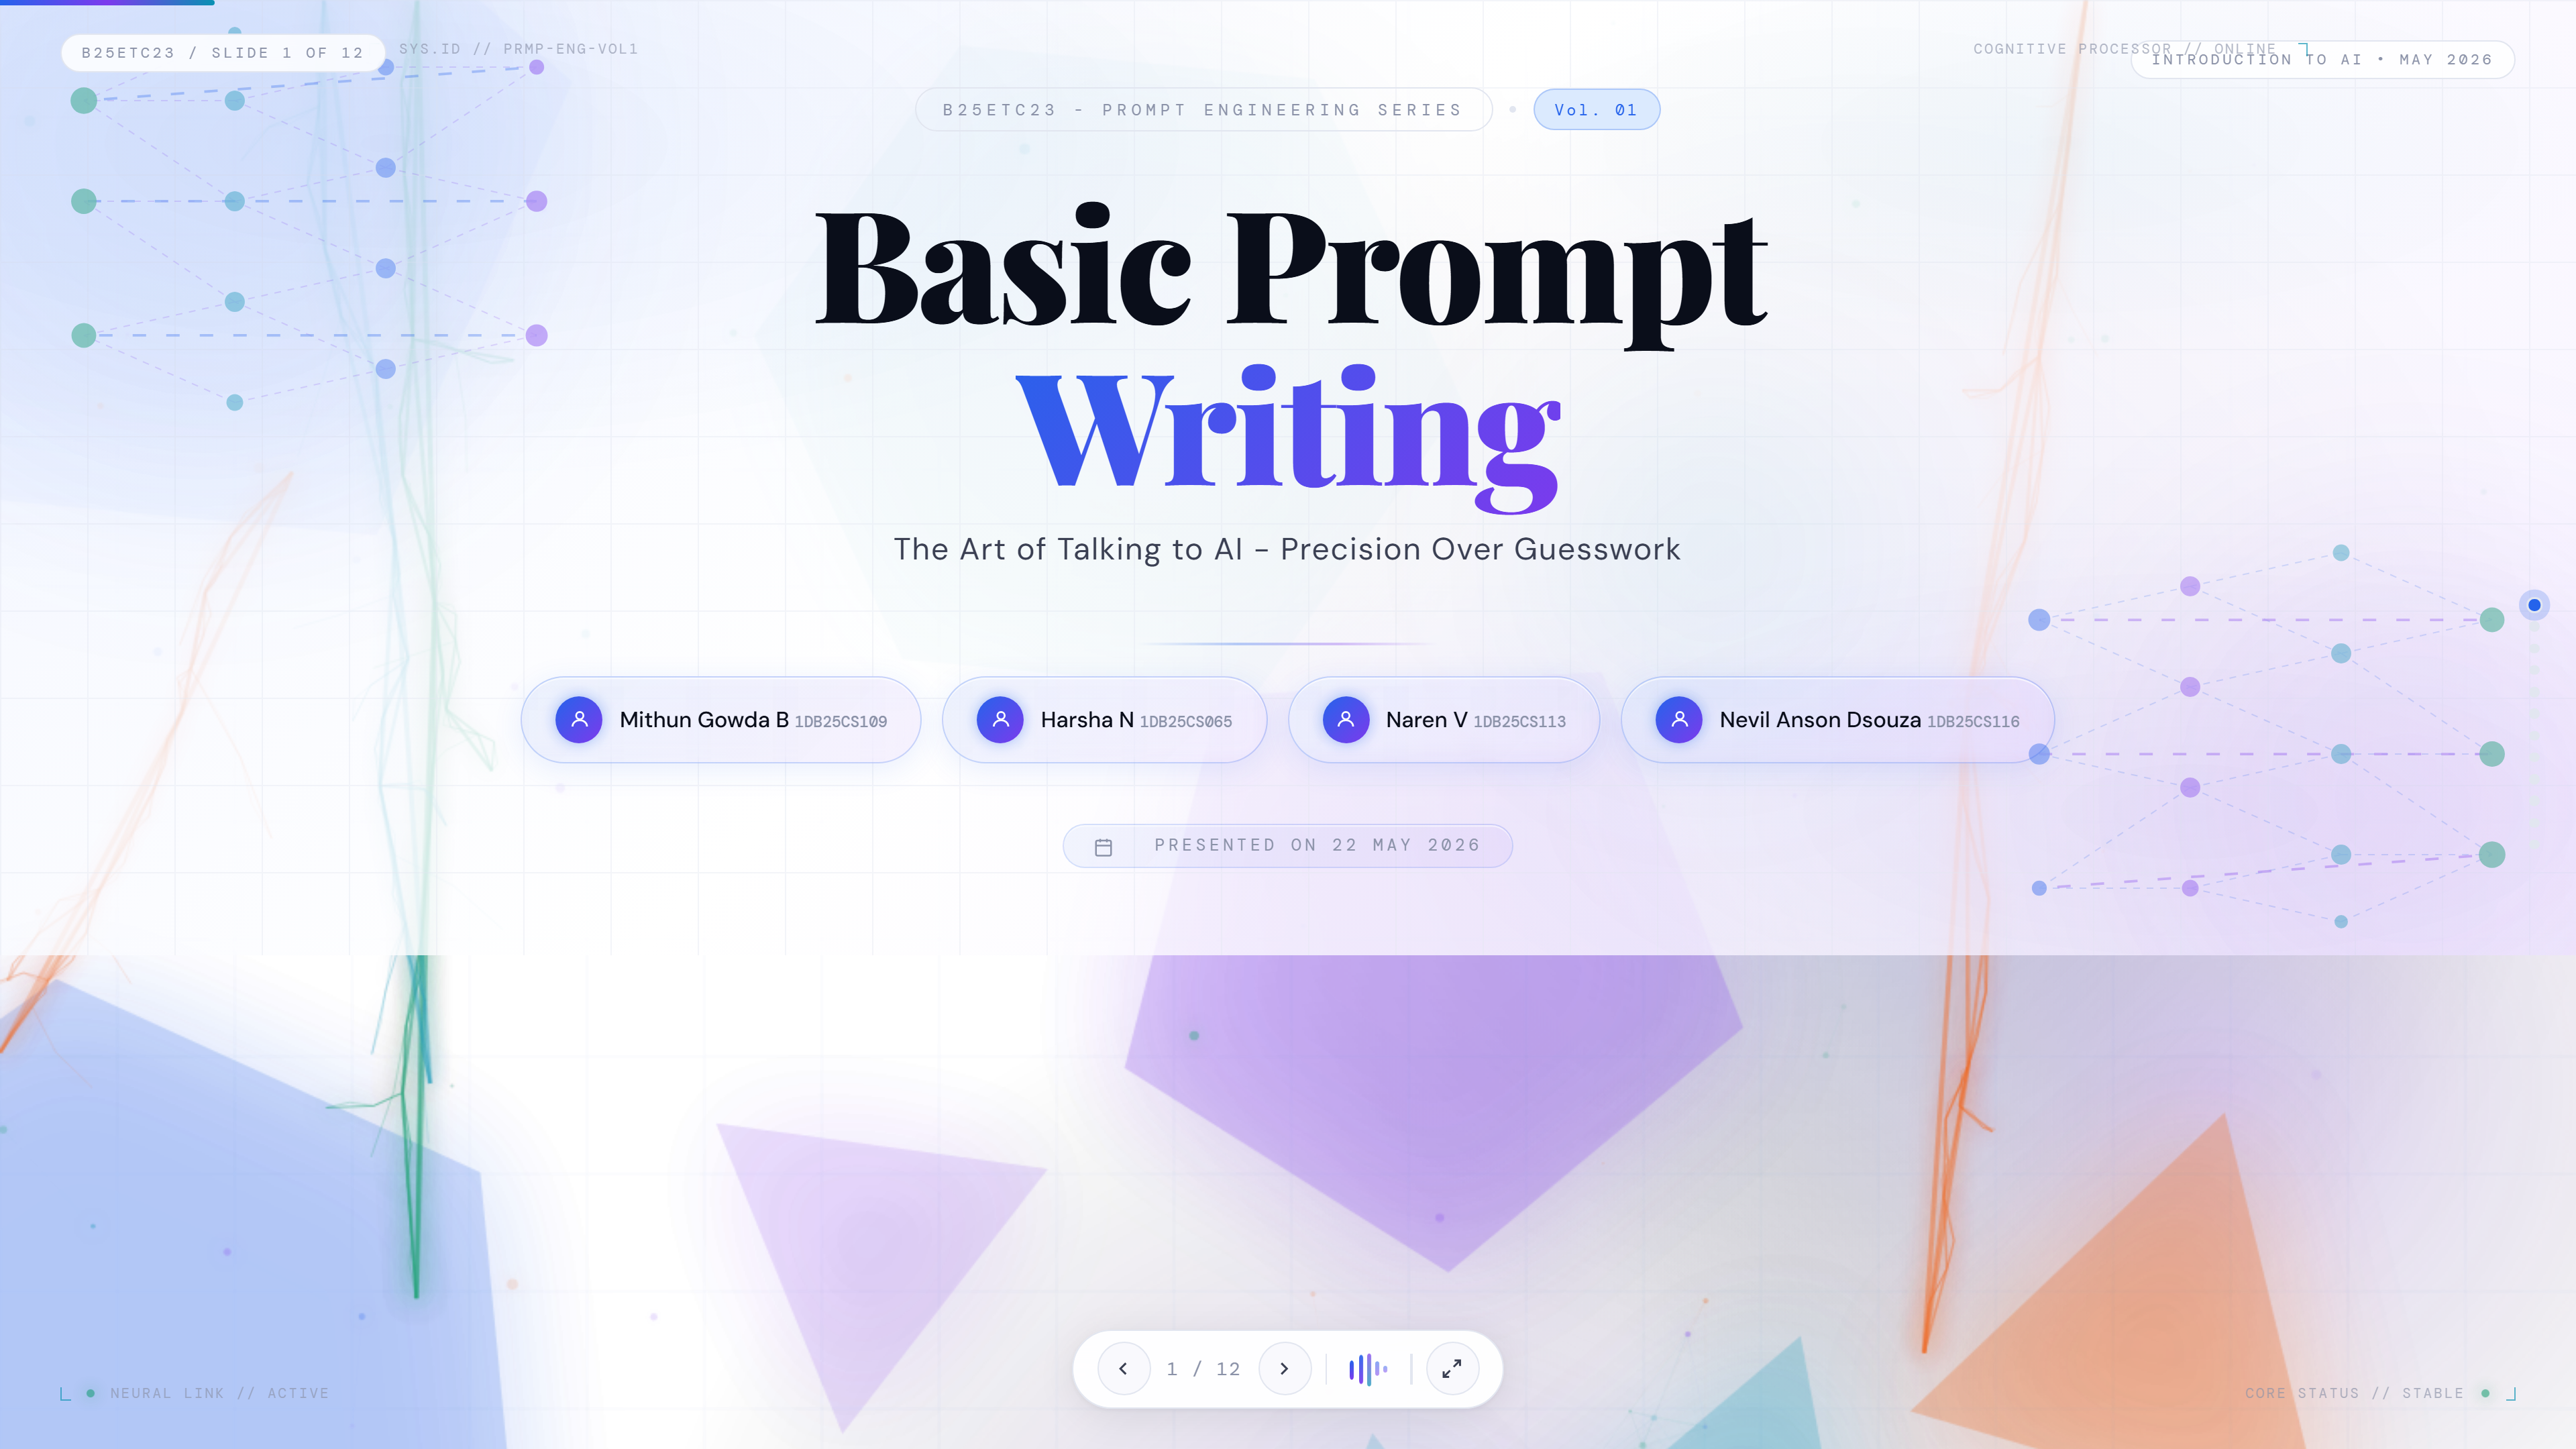
\includegraphics[width=0.92\textwidth]{slide_01.png}
  \caption{Slide 1: Title Slide -- Basic Prompt Writing}
\end{figure}

The title slide introduces the topic \emph{Basic Prompt Writing} under the B25ETC23 Introduction to AI course. The full subtitle -- \emph{The Art of Talking to AI: Precision Over Guesswork} -- frames the central question of the presentation: does it matter how you ask an AI a question? The slide identifies the four-member team and establishes the demonstration topic (Electricity) that will be used throughout.

\newpage

% ── Slide 2 ──
\subsection*{Slide 2 -- What is Prompt Engineering?}
\label{sec:s2}

\begin{figure}[H]
  \centering
  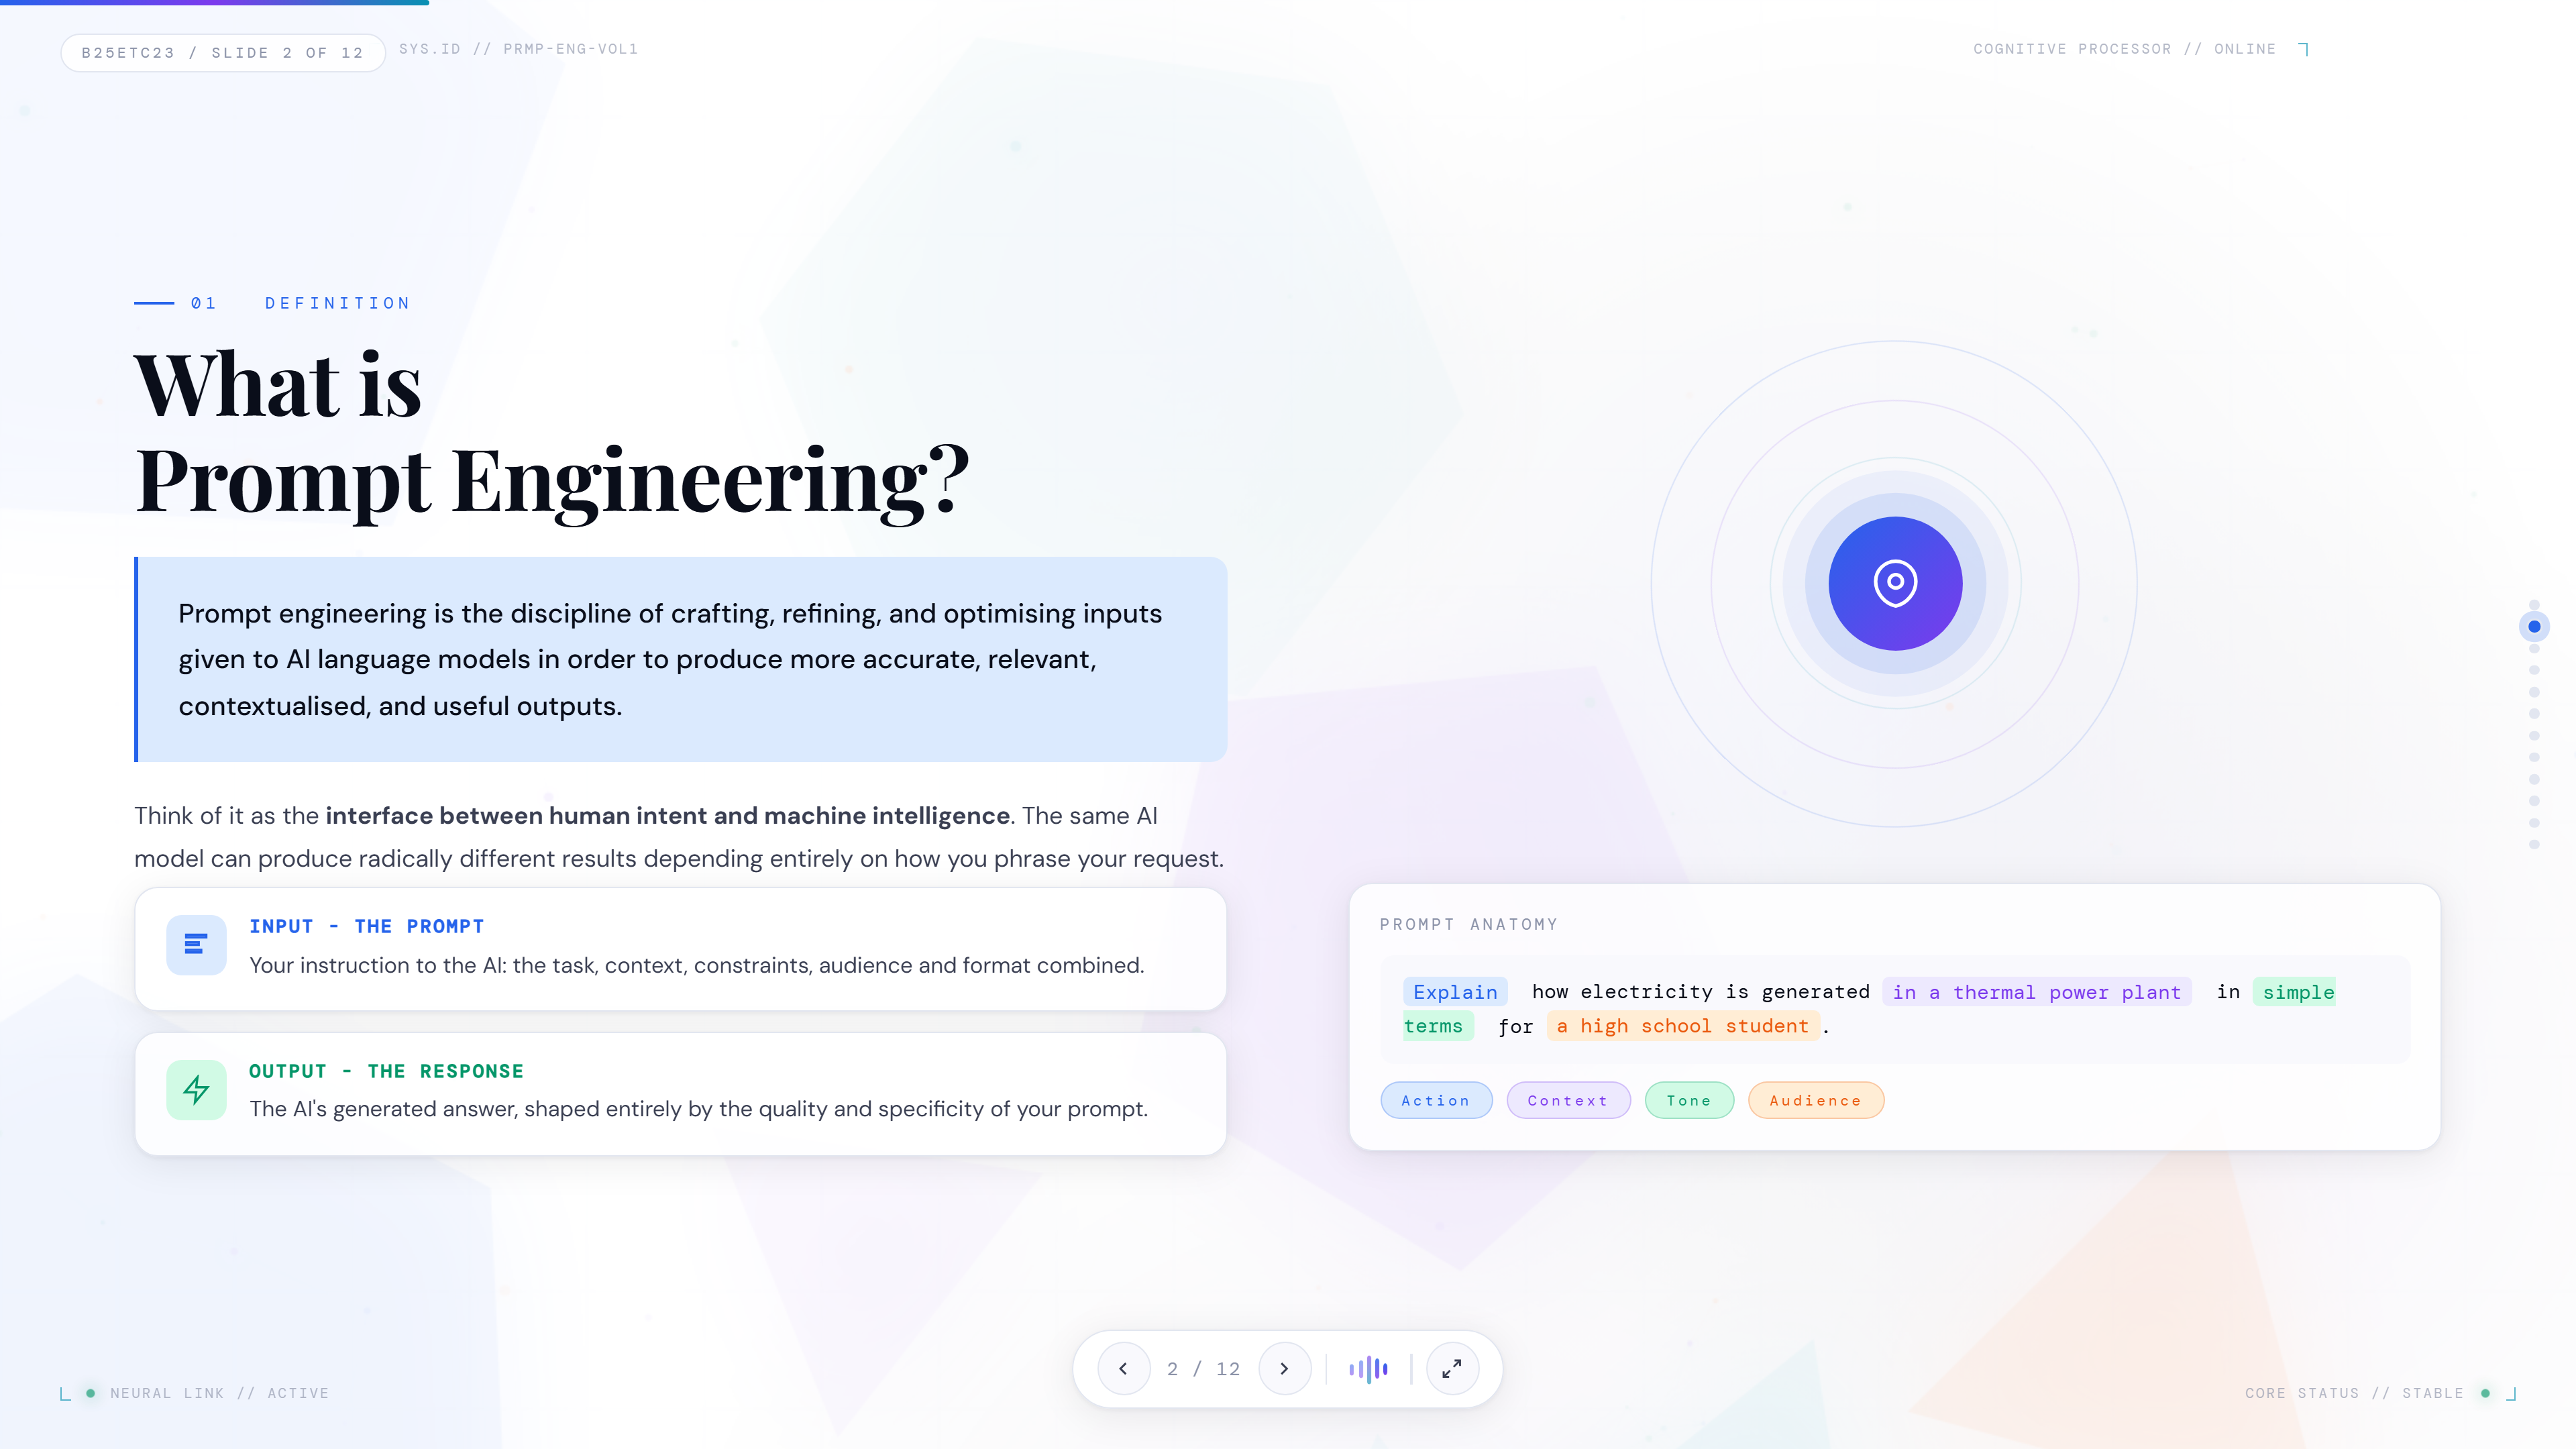
\includegraphics[width=0.92\textwidth]{slide_02.png}
  \caption{Slide 2: Definition and structure of a prompt}
\end{figure}

This slide defines what a prompt is and introduces prompt engineering as a discipline. The key analogy presented is that the AI model is a powerful engine, while the prompt is the steering wheel -- without good steering, even the most powerful engine goes nowhere useful. The slide shows an example of a well-structured prompt: \emph{``Explain how electricity is generated in a thermal power plant in simple terms for a high school student.''}

It breaks this into its components: an action (Explain), a context (thermal power plant), a tone (simple terms), and an audience (high school student). Every prompt has two parts -- the Input (your instruction combining task, context, audience, and format) and the Output (the AI response, entirely shaped by the quality of the input).

\newpage

% ── Slide 3 ──
\subsection*{Slide 3 -- Why Prompts Matter}
\label{sec:s3}

\begin{figure}[H]
  \centering
  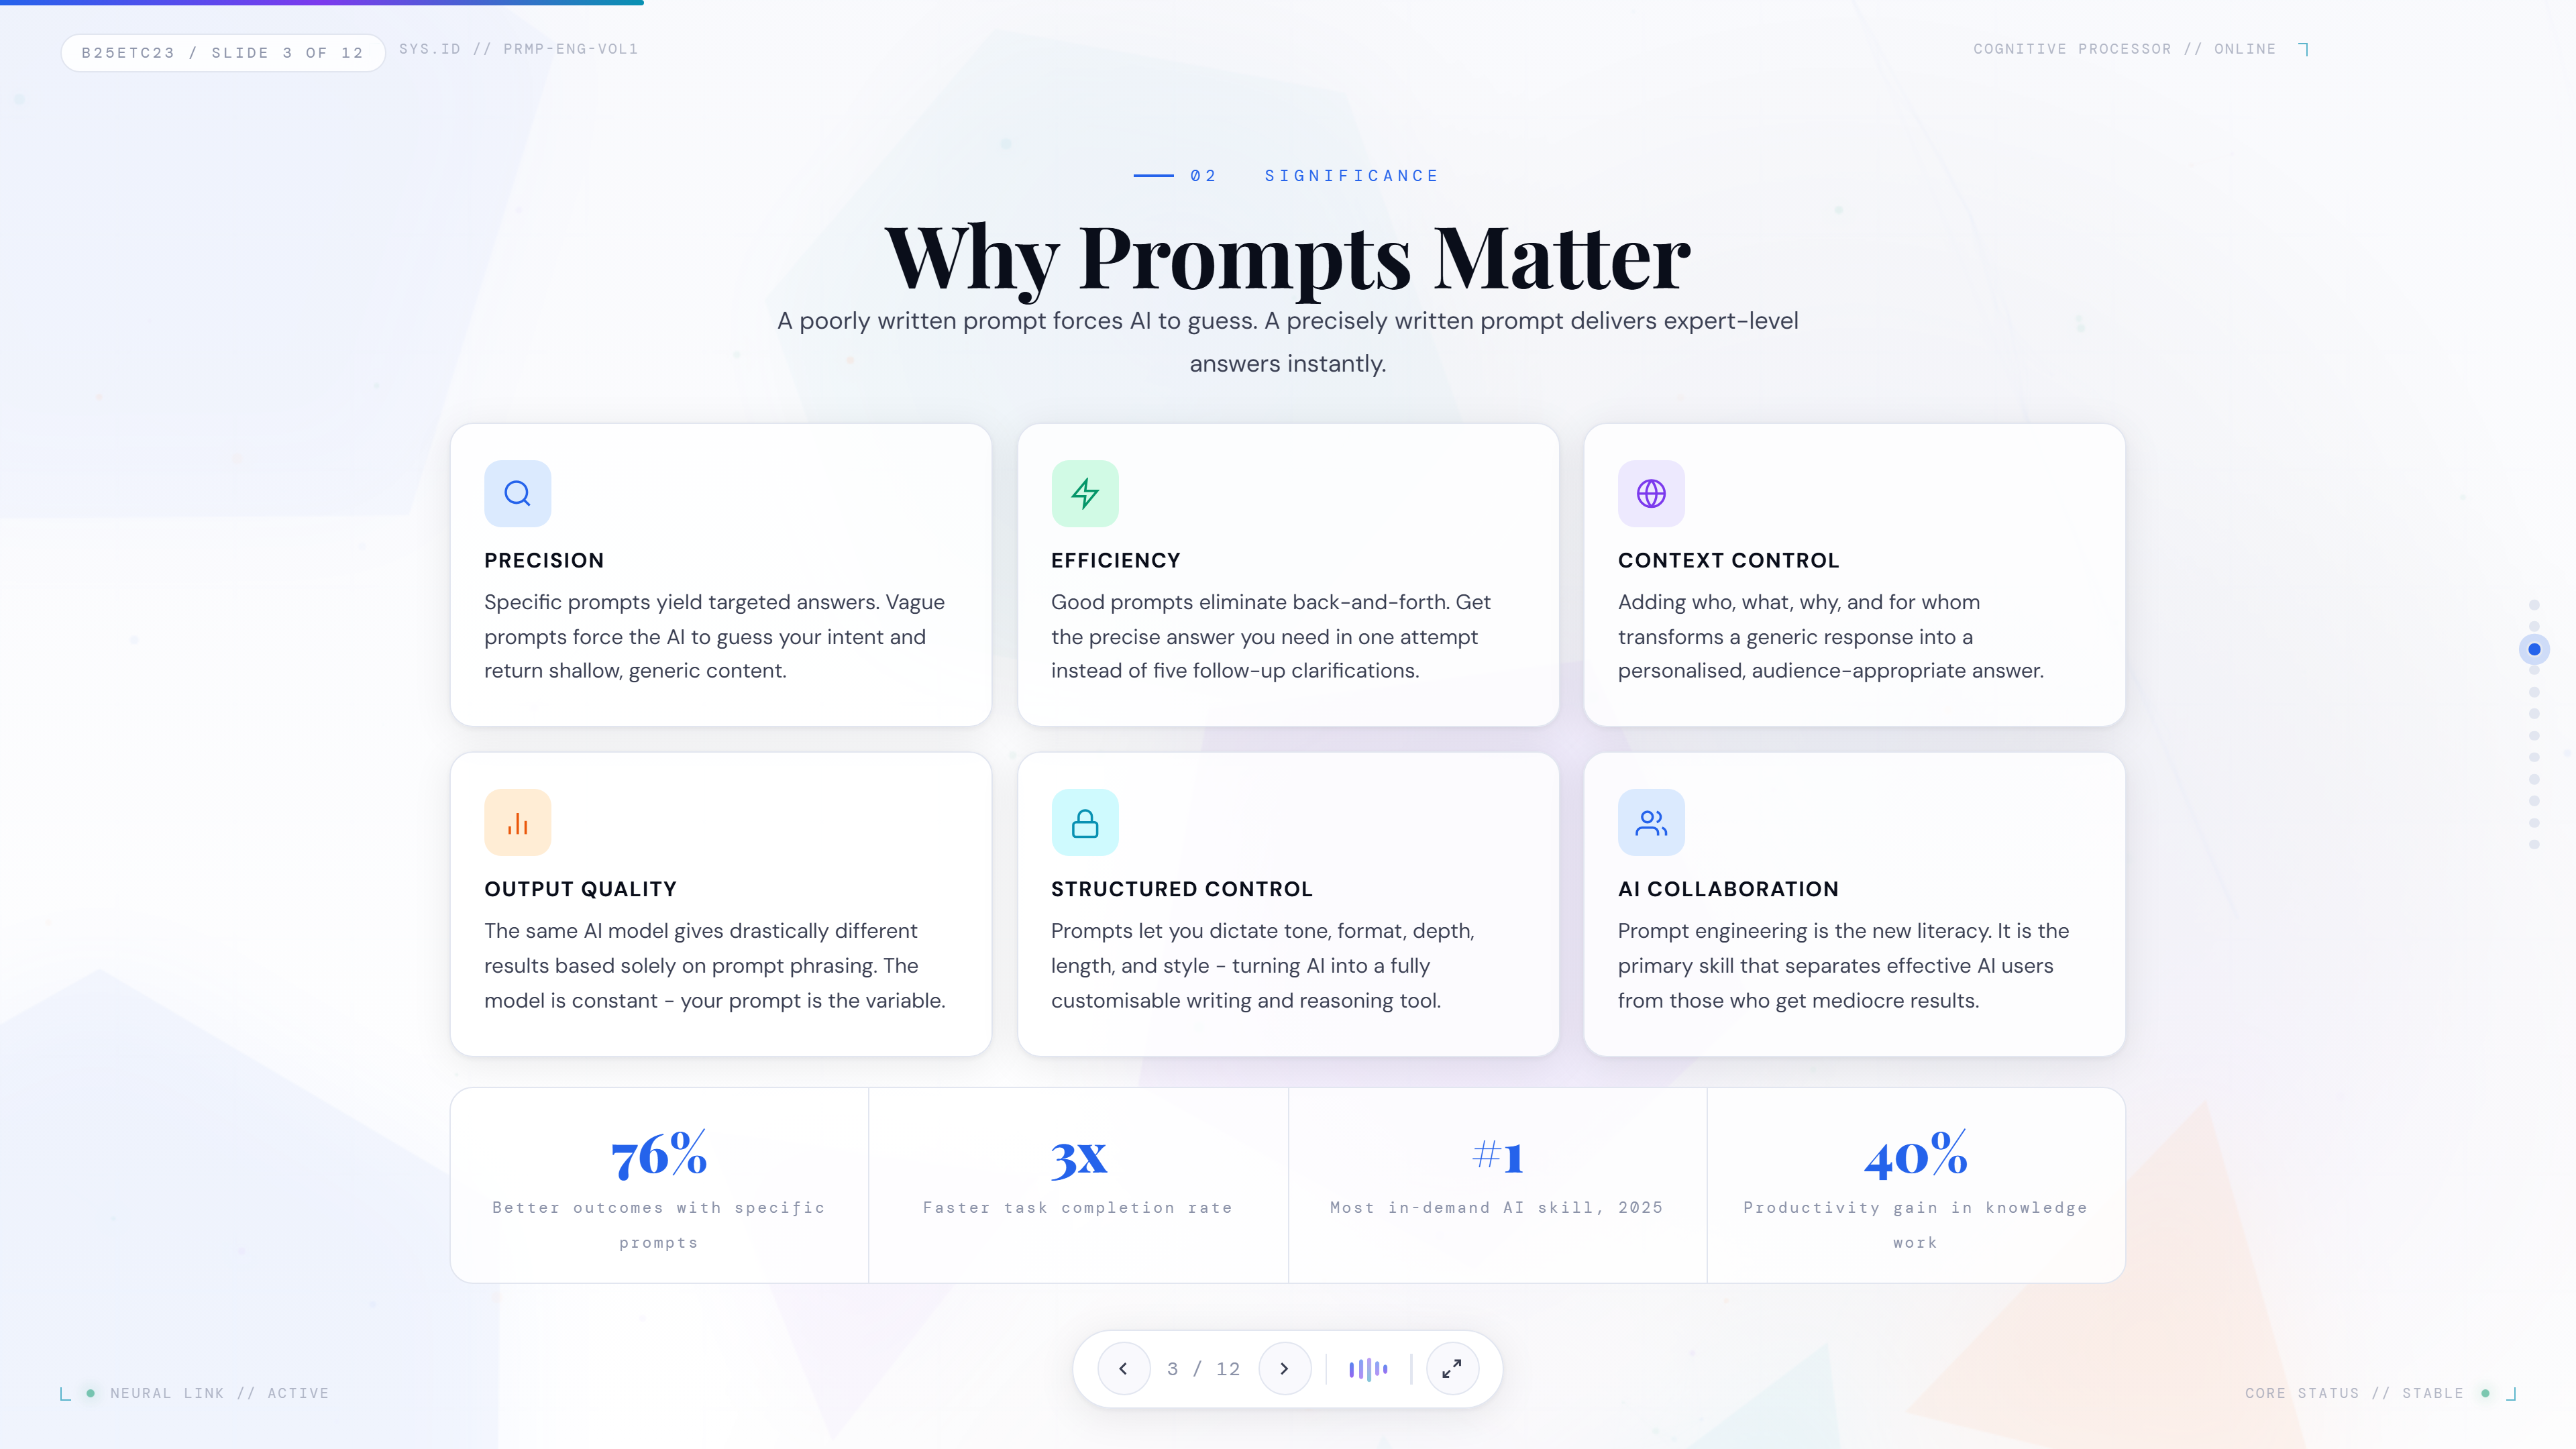
\includegraphics[width=0.92\textwidth]{slide_03.png}
  \caption{Slide 3: Six reasons why prompt quality matters}
\end{figure}

This slide presents six reasons why prompt engineering is critical:

\begin{enumerate}
  \item \textbf{Precision} -- Specific prompts give targeted answers; vague ones return shallow content.
  \item \textbf{Efficiency} -- A well-written prompt gets the answer in one shot instead of multiple follow-ups.
  \item \textbf{Context Control} -- Adding who the answer is for turns a generic response into a personalised one.
  \item \textbf{Output Quality} -- The model is constant; your prompt is the variable.
  \item \textbf{Structured Control} -- You can dictate tone, format, depth, and length.
  \item \textbf{AI Collaboration} -- Prompt engineering is the new literacy separating effective AI users from mediocre ones.
\end{enumerate}

Supporting statistics: 76\% better outcomes with specific prompts, 3x faster task completion, \#1 most in-demand AI skill in 2025, and 40\% productivity gain in knowledge work.

\newpage

% ── Slide 4 ──
\subsection*{Slide 4 -- The Electricity Experiment}
\label{sec:s4}

\begin{figure}[H]
  \centering
  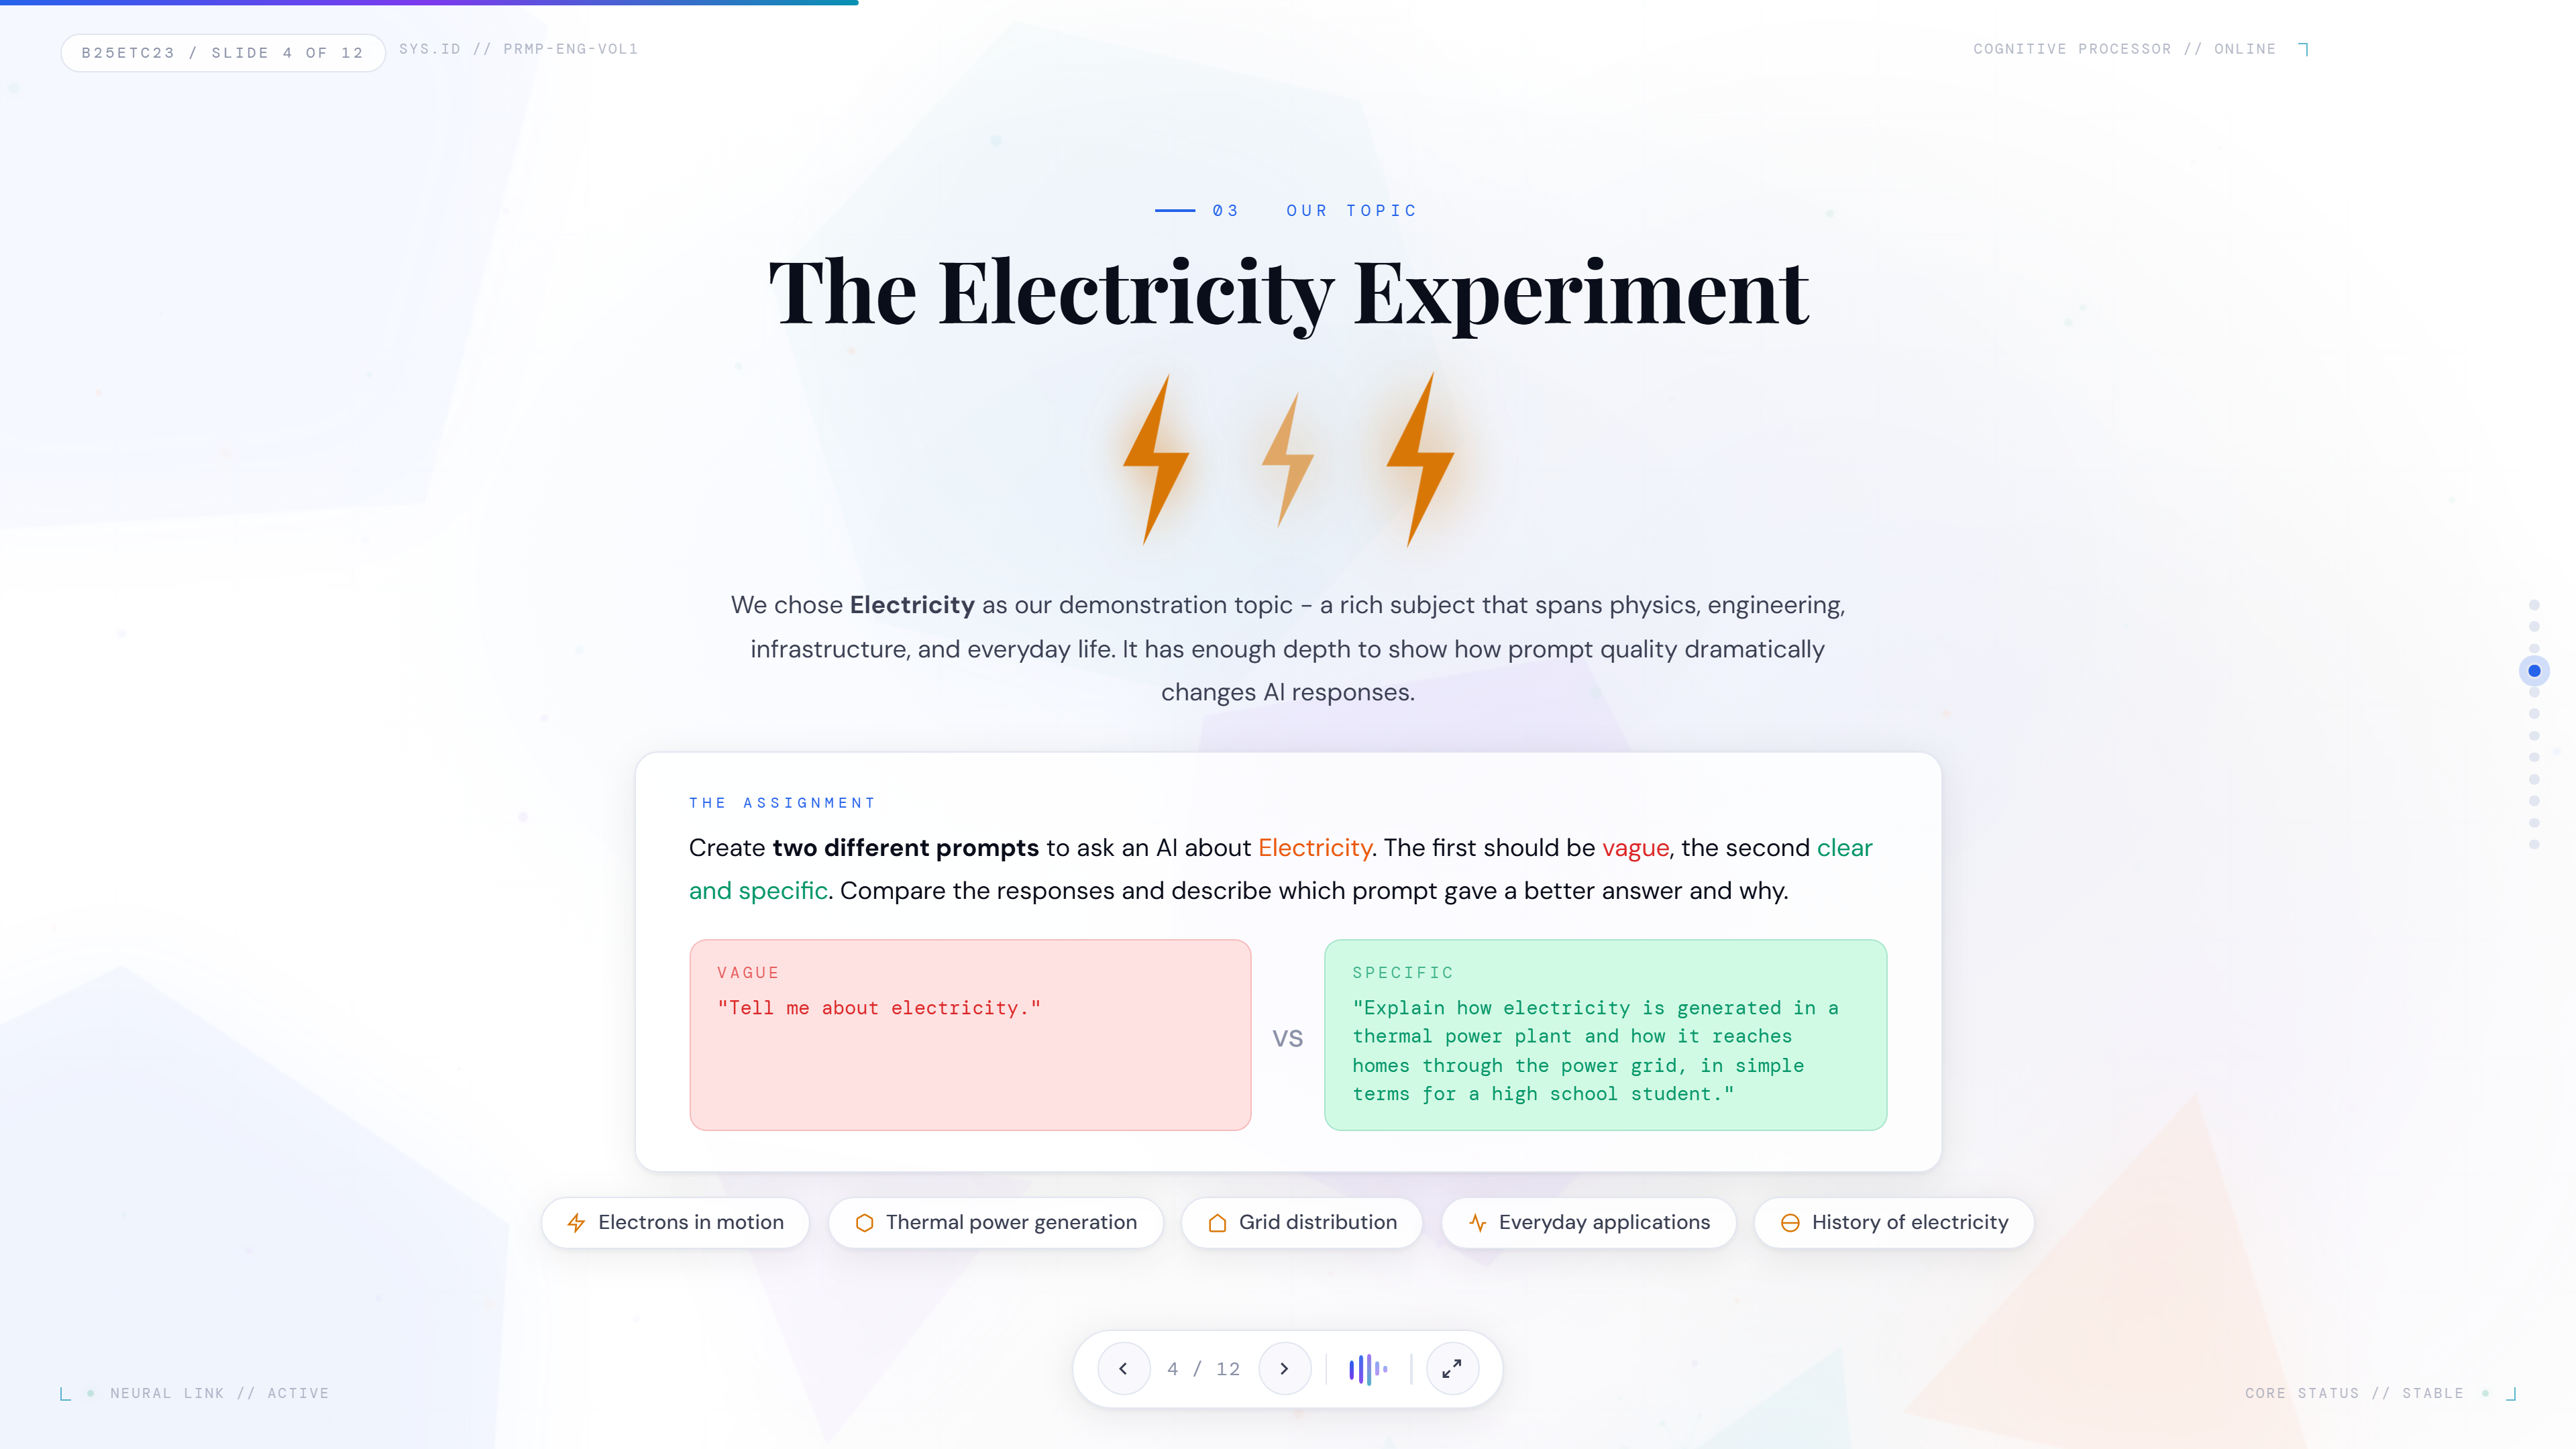
\includegraphics[width=0.92\textwidth]{slide_04.png}
  \caption{Slide 4: Experiment setup -- two prompts on Electricity}
\end{figure}

This slide introduces the experiment. The assignment was to create two different prompts about Electricity -- one vague, one specific -- and compare the AI responses.

\textbf{Prompt 1 -- Vague:} \emph{``Tell me about electricity.''}

\textbf{Prompt 2 -- Specific:} \emph{``Explain how electricity is generated in a thermal power plant and how it reaches homes through the power grid, in simple terms for a high school student.''}

Electricity was chosen as the demonstration topic because it is a rich subject spanning physics, engineering, infrastructure, and everyday life -- with enough depth and breadth to clearly show how prompt quality changes AI responses.

\newpage

% ── Slide 5 ──
\subsection*{Slide 5 -- The Vague Prompt Response}
\label{sec:s5}

\begin{figure}[H]
  \centering
  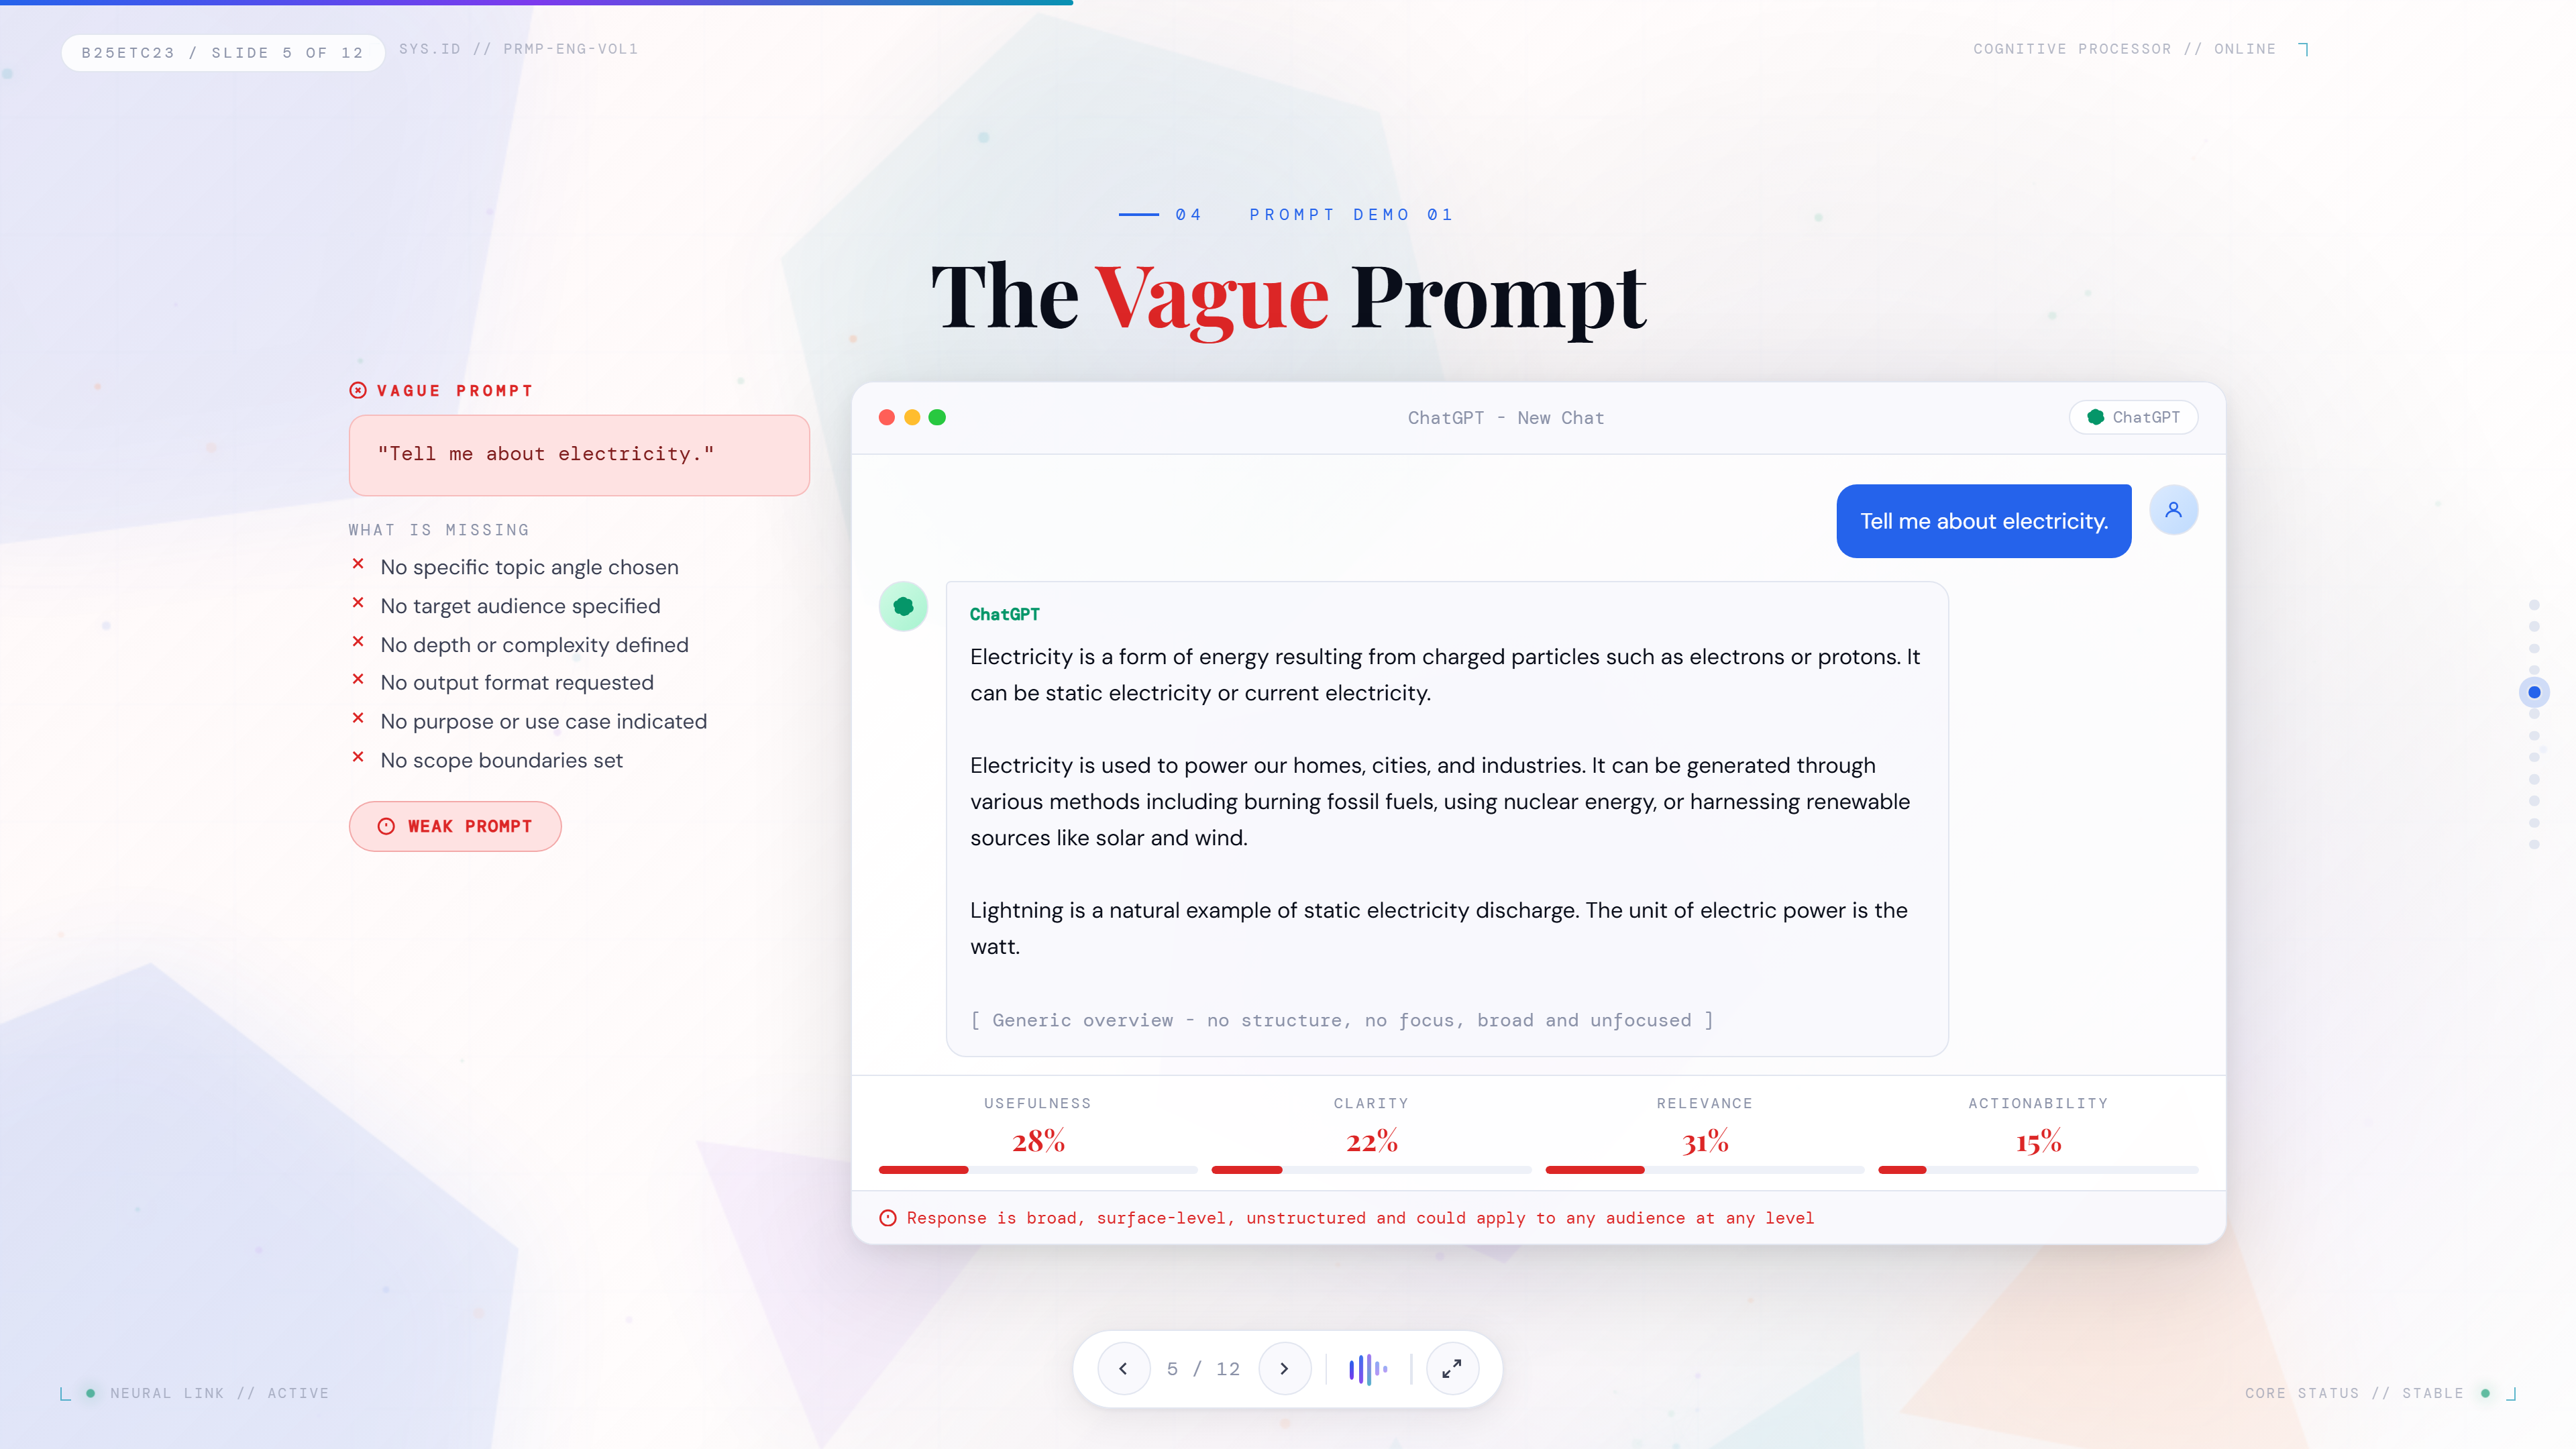
\includegraphics[width=0.92\textwidth]{slide_05.png}
  \caption{Slide 5: ChatGPT response to the vague prompt}
\end{figure}

This slide shows the actual ChatGPT response to \emph{``Tell me about electricity.''}

The response is a generic overview: it defines electricity, mentions static and current electricity, lists power sources (fossil fuels, nuclear, solar, wind), and references lightning. What is wrong with this response:

\begin{itemize}
  \item Generic overview -- no structure, no logical flow
  \item Mixes unrelated topics: static electricity, lightning, solar, nuclear -- all jumbled together
  \item Written for nobody in particular -- not a student, not an engineer, not a child
  \item Cannot be directly used in any assignment or report
\end{itemize}

Analysis scores confirm this: \textbf{Usefulness 28\%, Clarity 22\%, Relevance 31\%, Actionability 15\%.}

\newpage

% ── Slide 6 ──
\subsection*{Slide 6 -- The Specific Prompt Response}
\label{sec:s6}

\begin{figure}[H]
  \centering
  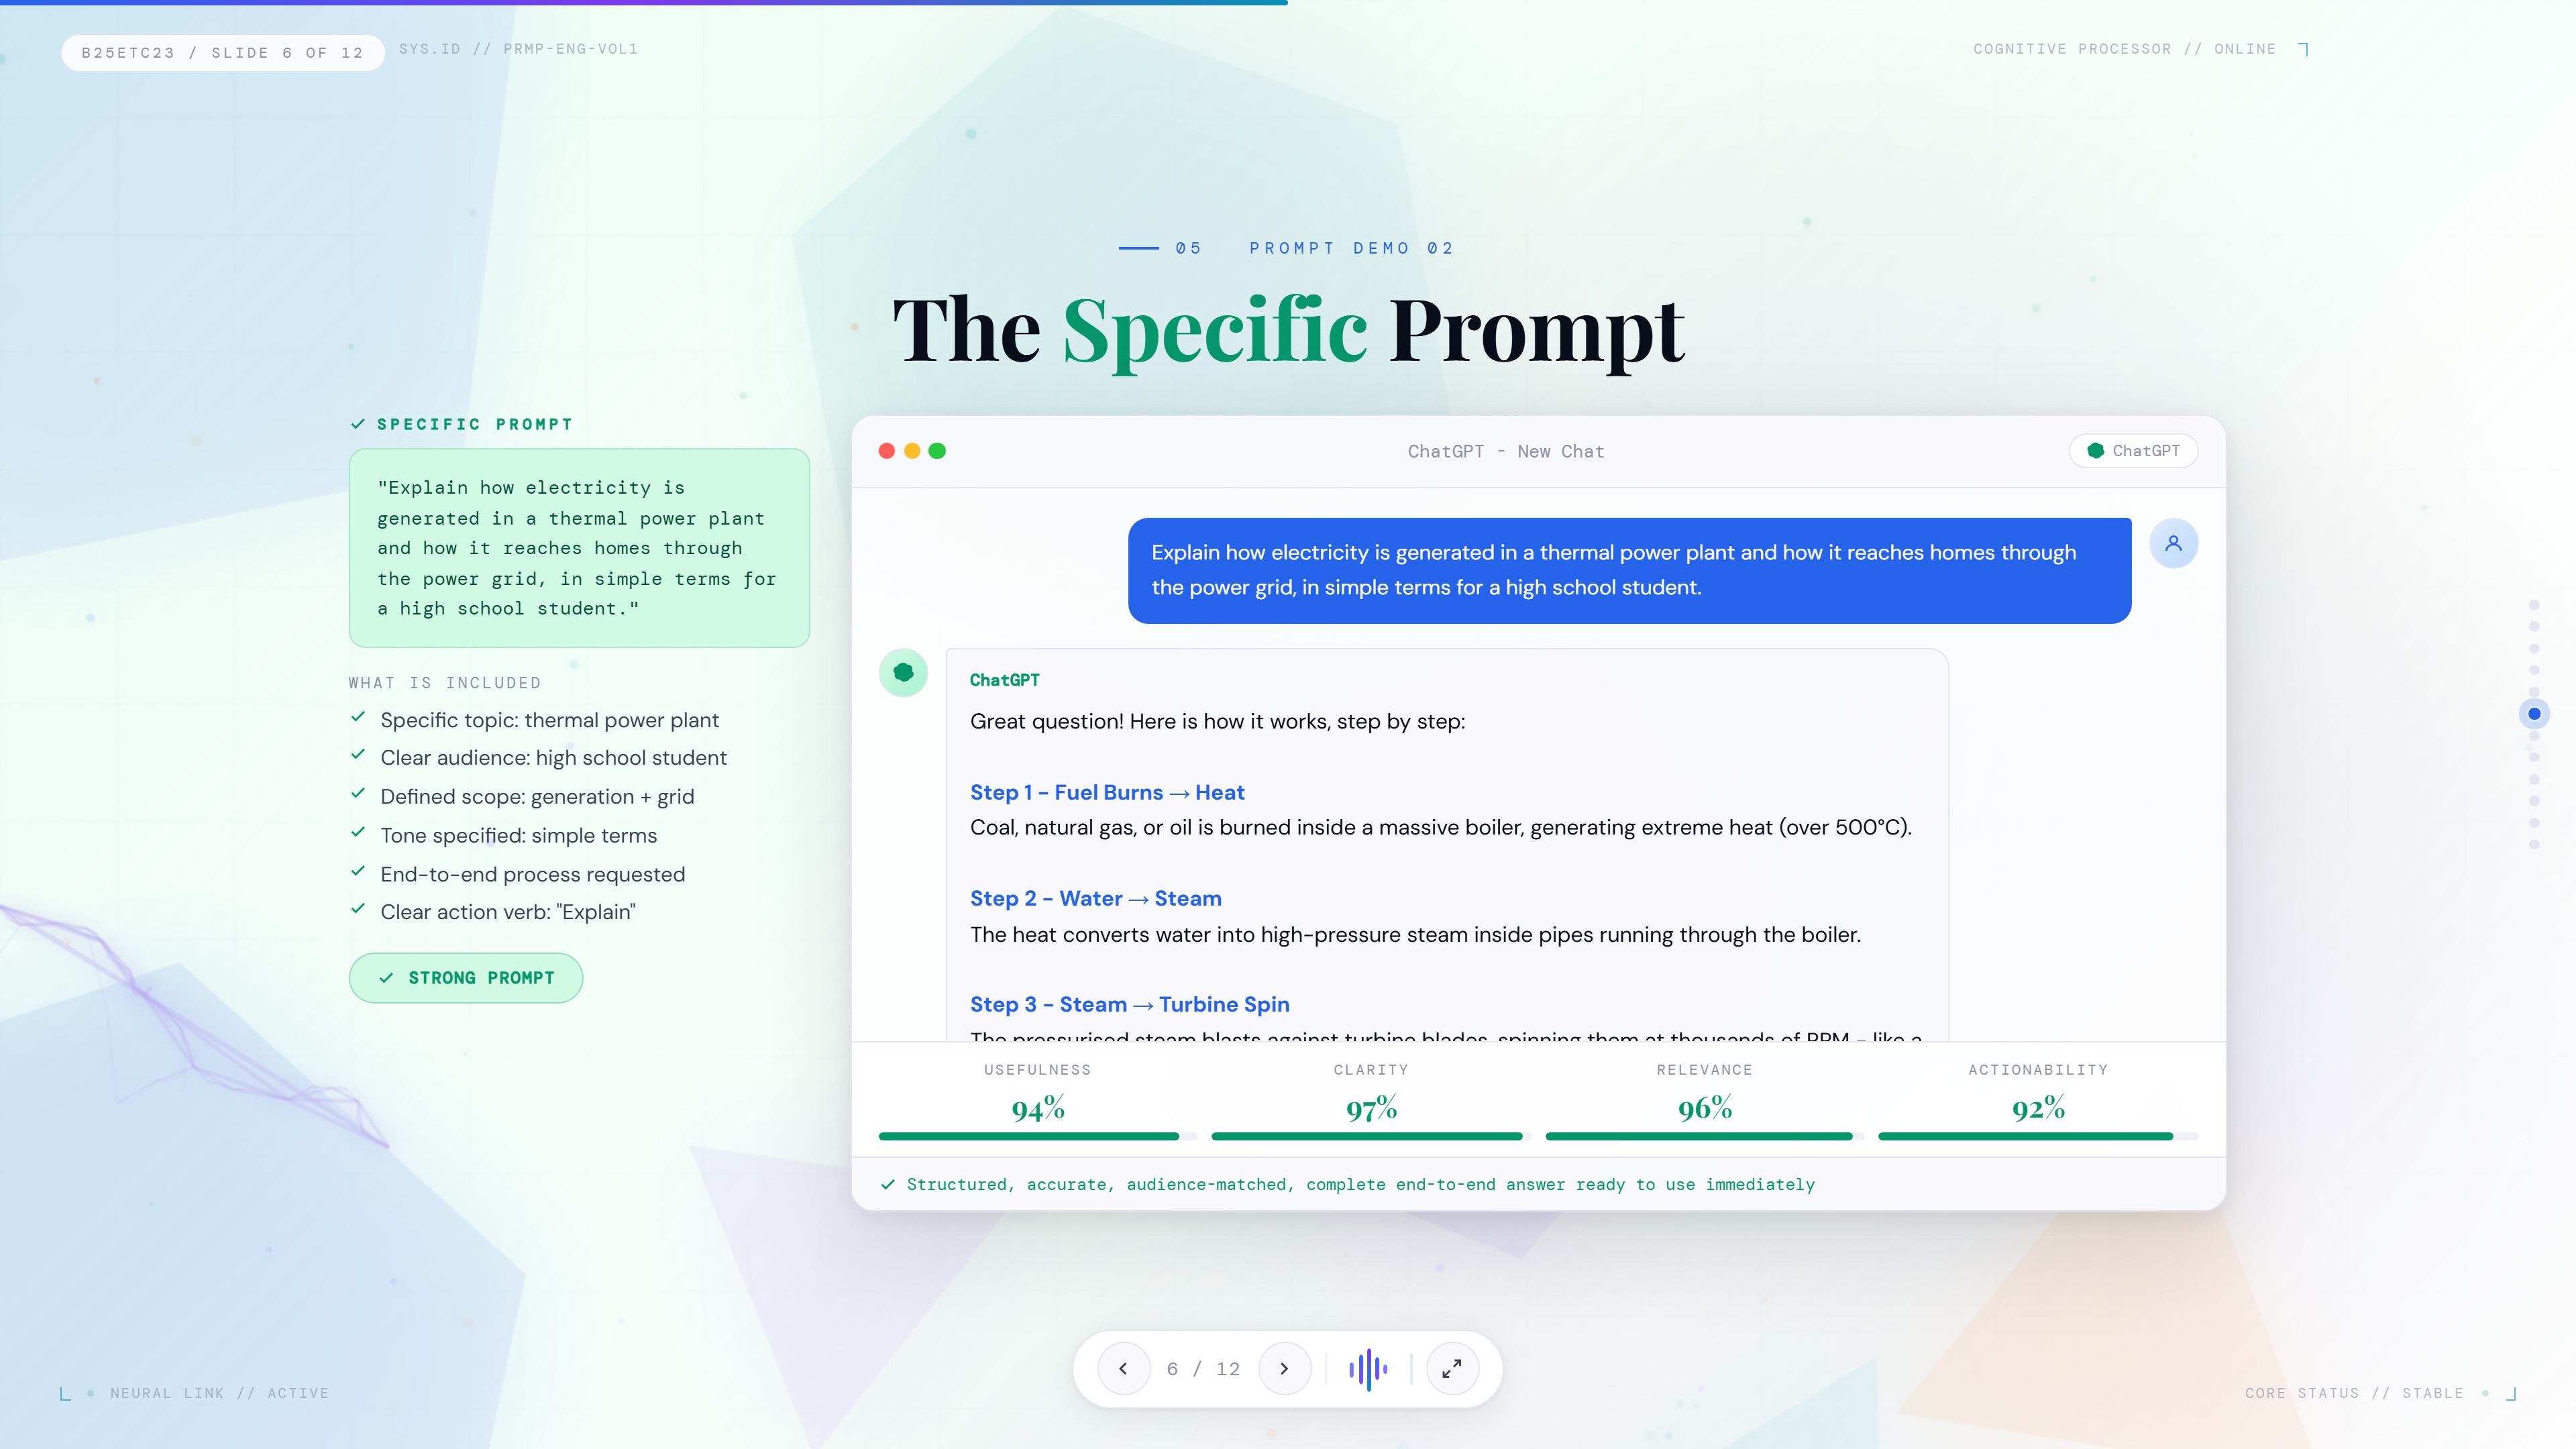
\includegraphics[width=0.92\textwidth]{slide_06.png}
  \caption{Slide 6: ChatGPT response to the specific prompt}
\end{figure}

This slide shows the ChatGPT response to the specific prompt. The difference is dramatic. The AI delivered a structured 6-step process:

\begin{enumerate}
  \item \textbf{Fuel Burns, Heat is Produced} -- Coal or gas burned in a boiler above 500 degrees Celsius.
  \item \textbf{Heat Turns Water into Steam}
  \item \textbf{Steam Spins a Turbine} -- Like a jet engine, at thousands of RPM.
  \item \textbf{Turbine Spins a Generator} -- Magnets rotating inside copper coils create electricity through electromagnetic induction.
  \item \textbf{Transformer Steps Up Voltage} -- To 400,000V for efficient long-distance transmission.
  \item \textbf{Substation Brings it Down} -- Back to 230V before it enters your home.
\end{enumerate}

The response is focused, structured, audience-appropriate, and immediately usable. Scores: \textbf{Usefulness 94\%, Clarity 97\%, Relevance 96\%, Actionability 92\%.}

Same AI. Same topic. Completely different quality -- because of the prompt alone.

\newpage

% ── Slide 7 ──
\subsection*{Slide 7 -- Side-by-Side Comparison}
\label{sec:s7}

\begin{figure}[H]
  \centering
  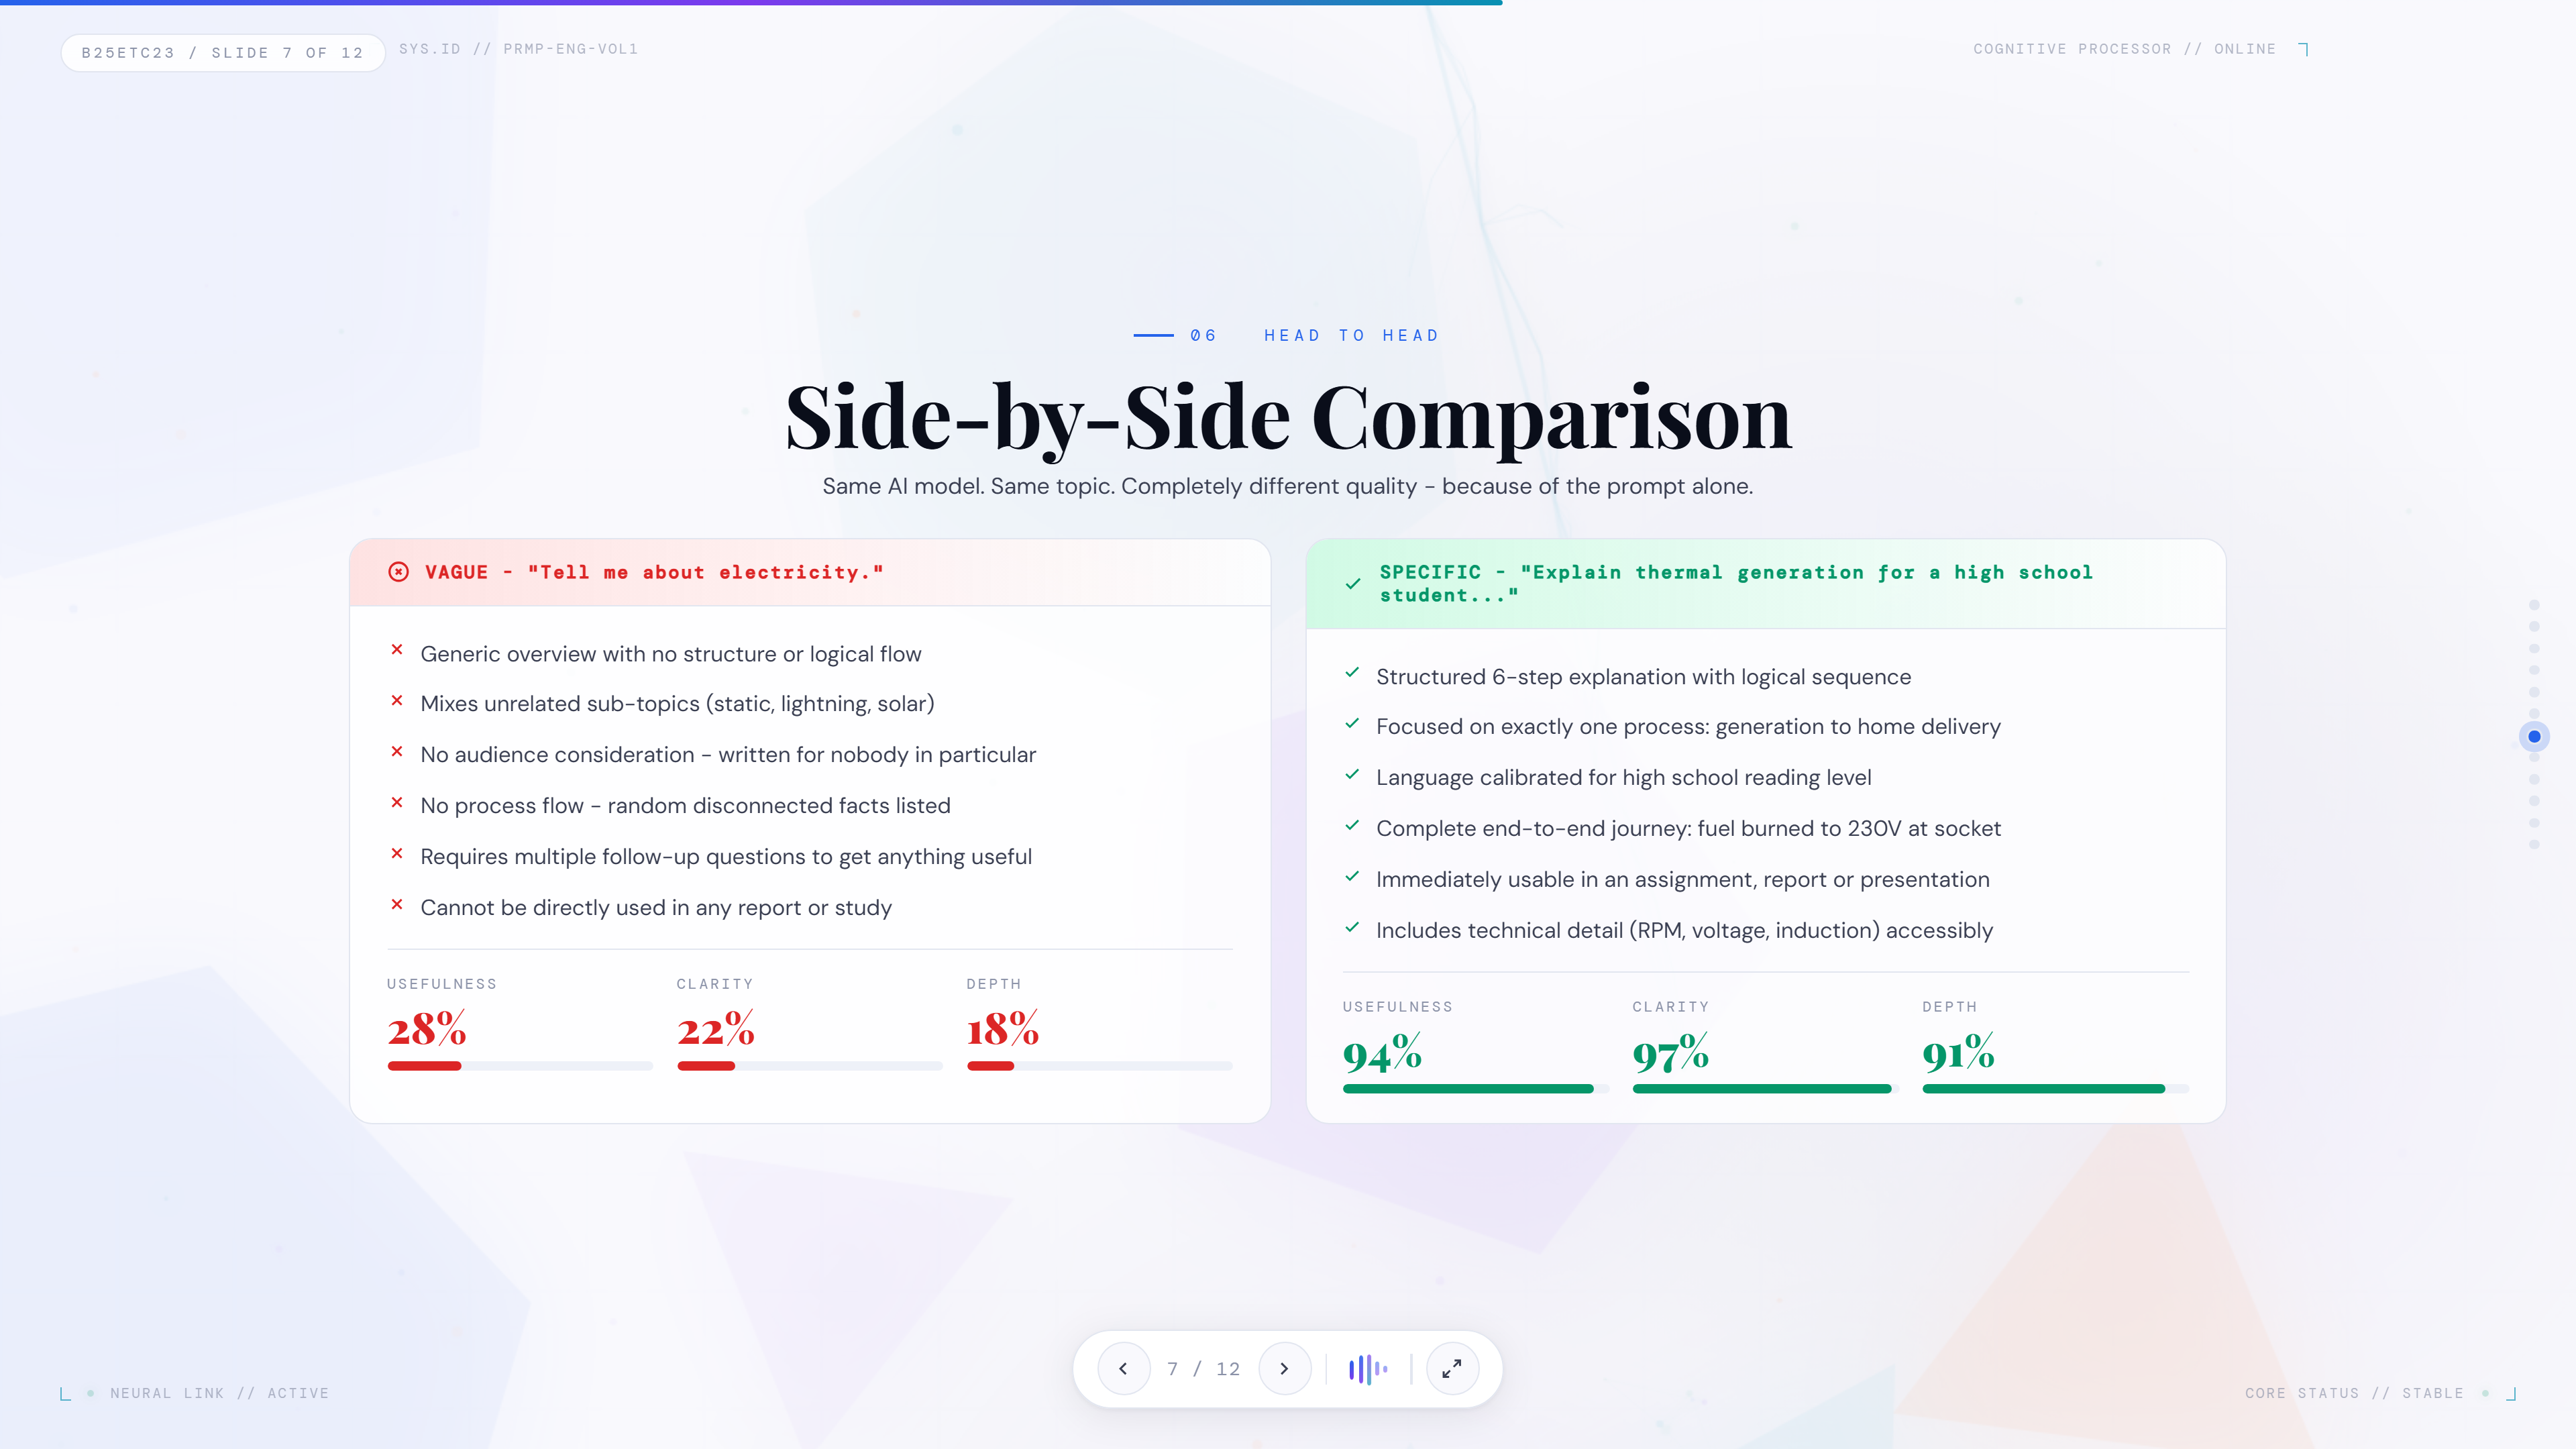
\includegraphics[width=0.92\textwidth]{slide_07.png}
  \caption{Slide 7: Direct comparison of both responses}
\end{figure}

This slide places both responses side by side for direct comparison.

\textbf{Vague prompt response:}
\begin{itemize}
  \item Generic overview with no structure
  \item Mixes unrelated sub-topics
  \item No audience consideration
  \item Random disconnected facts
  \item Requires multiple follow-up questions
  \item Scores: Usefulness 28\%, Clarity 22\%, Depth 18\%
\end{itemize}

\textbf{Specific prompt response:}
\begin{itemize}
  \item Structured 6-step logical sequence
  \item Focused on one clearly defined process
  \item Language calibrated for high school level
  \item Complete end-to-end journey from fuel to socket
  \item Immediately usable in an assignment or presentation
  \item Scores: Usefulness 94\%, Clarity 97\%, Depth 91\%
\end{itemize}

The key insight: \textbf{the AI model did not change.} The entire difference came from the prompt alone.

To put the numbers in perspective, the vague prompt scored an average of 24\% across all quality dimensions, while the specific prompt scored an average of 94.75\%. This means the specific prompt produced a response that was nearly four times more effective than the vague prompt -- using the exact same AI system, in the same session, with no changes to the model configuration or parameters.

The vague response reads like a dictionary entry -- a flat collection of facts with no narrative, no purpose, and no intended reader. It tells you what electricity is, but it does not help you understand how it works, why it matters, or how it reaches your home. A student reading this response would still need to ask five or six follow-up questions to get any useful information, making the initial prompt effectively useless.

The specific response, on the other hand, reads like a well-planned lesson. It starts at the beginning of the process (fuel burning), follows a logical sequence through each stage of electricity generation and transmission, and ends at the point of use (your wall socket). Each step builds on the previous one. Technical terms like ``electromagnetic induction'' are introduced naturally and explained in context. The response is complete enough to stand alone as a learning resource.

This comparison demonstrates a critical principle of AI interaction: \textbf{the quality of the question determines the quality of the answer}. Users who blame the AI for poor responses are often, unknowingly, blaming their own prompts. The AI is not the bottleneck -- the prompt is. This is both the challenge and the opportunity of prompt engineering: the power to improve AI output is entirely in the user's hands.

\newpage

% ── Slide 8 ──
\subsection*{Slide 8 -- Why the Specific Prompt Succeeded}
\label{sec:s8}

\begin{figure}[H]
  \centering
  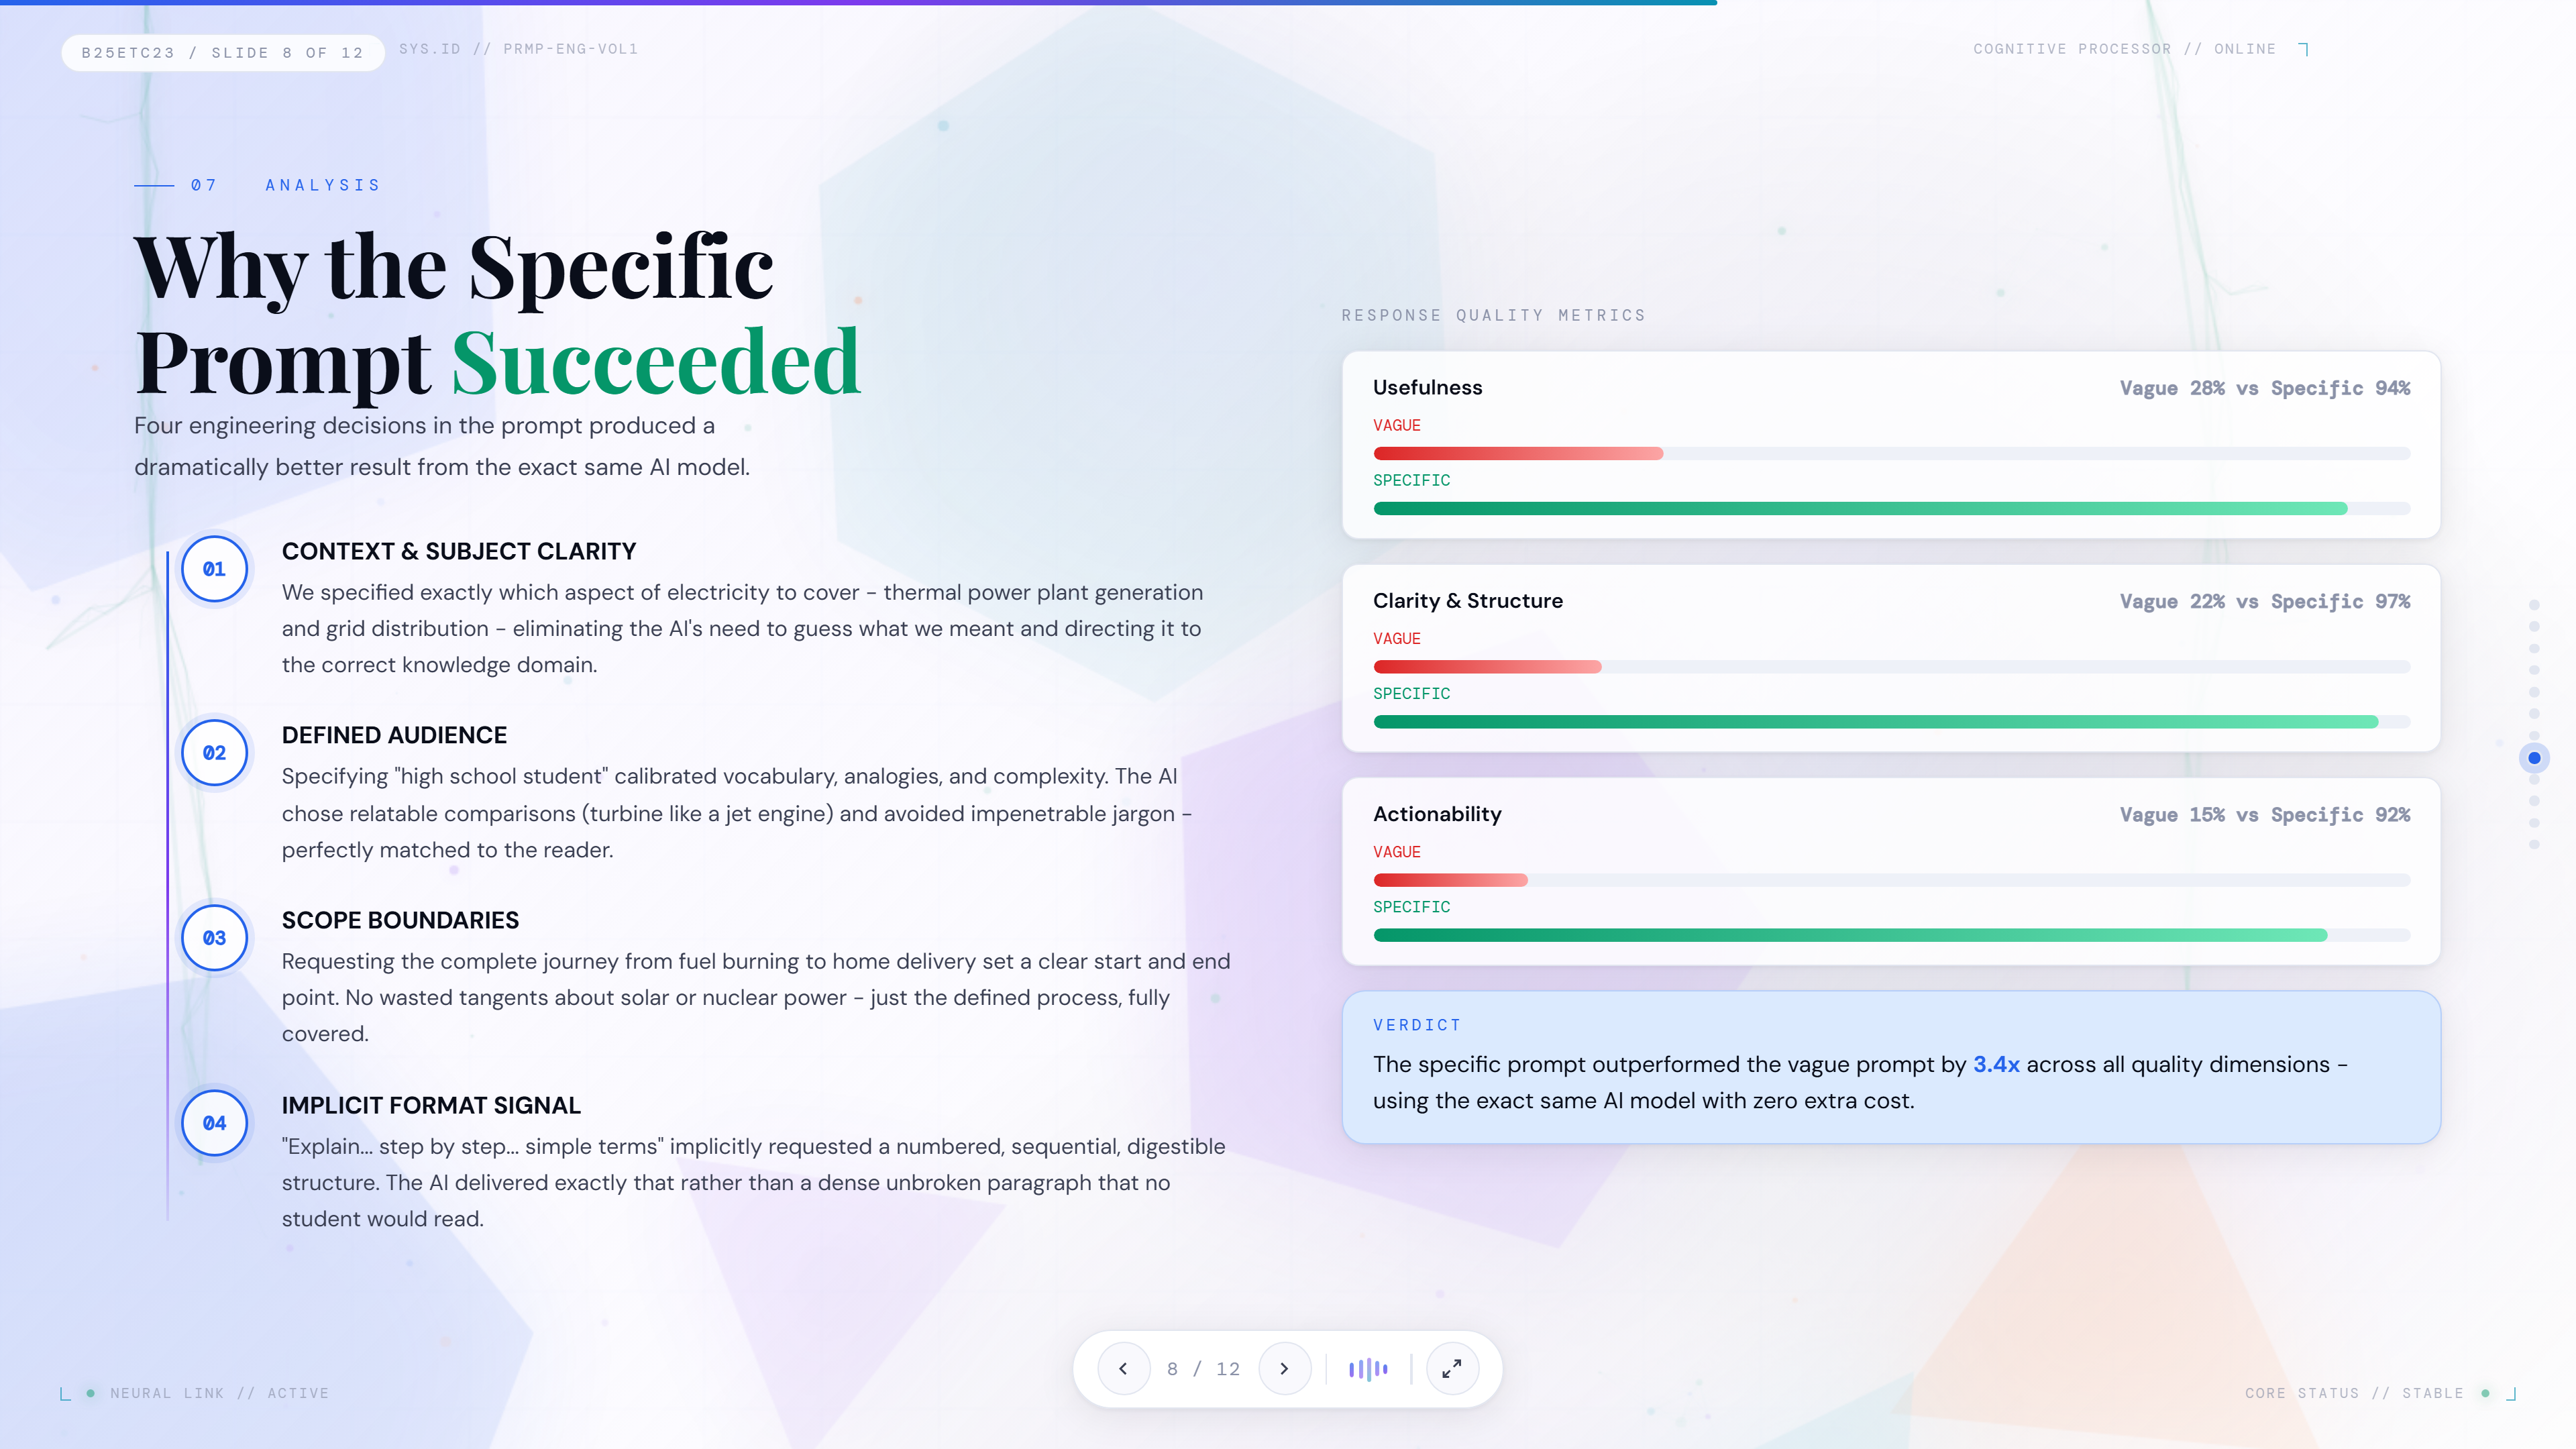
\includegraphics[width=0.92\textwidth]{slide_08.png}
  \caption{Slide 8: Four factors behind the specific prompt's success}
\end{figure}

This slide analyses the four deliberate decisions inside the specific prompt that drove its superior performance. Each decision addresses a specific weakness that was present in the vague prompt:

\begin{enumerate}
  \item \textbf{Context and Subject Clarity} -- The vague prompt (``Tell me about electricity'') left the AI with no guidance on which aspect of a massive topic to address. The specific prompt told the AI exactly what to focus on: thermal power plant generation and grid distribution. This single change eliminated any guesswork about which corner of a huge topic to address, and prevented the AI from scattering its response across unrelated sub-topics like static electricity, lightning, or nuclear power.

  \item \textbf{Defined Audience} -- The phrase ``high school student'' calibrated everything about the response -- vocabulary, analogies, complexity level, and assumed prior knowledge. The AI chose relatable comparisons, like comparing the turbine to a jet engine, and avoided technical jargon that would confuse a student. Without this cue, the AI defaulted to writing for a generic adult reader, producing content that was too shallow for an expert but too dense for a student.

  \item \textbf{Scope Boundaries} -- Asking for the complete journey from fuel burning to home delivery set a clear start point and end point for the response. This prevented the AI from going off on tangents about solar power, nuclear energy, or lightning -- all of which appeared in the vague prompt response. The bounded scope forced the AI to cover one process completely rather than many processes superficially.

  \item \textbf{Implicit Format Signal} -- The phrase ``explain in simple terms'' implicitly asked for a structured, step-by-step breakdown rather than a dense academic paragraph. The AI interpreted this as a cue to use numbered steps with clear headings, making the response scannable and easy to follow. The vague prompt gave no format signal, so the AI defaulted to an unstructured prose paragraph that was difficult to extract information from.
\end{enumerate}

The combined effect of these four decisions was transformative. The specific prompt outperformed the vague one by \textbf{3.4 times} across all quality dimensions. What makes this finding particularly powerful is that none of these four elements required technical knowledge or AI expertise -- they are basic communication principles that anyone can apply.

\begin{table}[H]
\centering
\begin{tabular}{p{3.5cm}p{4cm}p{4cm}}
\toprule
\textbf{Factor} & \textbf{Vague Prompt (Missing)} & \textbf{Specific Prompt (Present)} \\
\midrule
Context & No topic angle specified & Thermal power plant + grid distribution \\
Audience & No target reader defined & High school student \\
Scope & Open-ended, unbounded & Fuel burning to home delivery \\
Format & No structure requested & Implicit step-by-step breakdown \\
\bottomrule
\end{tabular}
\caption{Comparison of prompt factors between vague and specific prompts}
\end{table}

The 3.4x improvement was not driven by any single factor alone -- it was the combination of all four working together that produced the dramatic difference. This is consistent with the CATO framework introduced in the next slide: each element (Context, Action, Target Audience, Output Format) contributes independently, but their combined effect is multiplicative rather than additive.

A key practical insight from this analysis is the concept of ``prompt cost.'' The vague prompt cost the user zero effort to write -- just four words. The specific prompt required approximately 25 words and a few seconds of additional thought. That marginal effort yielded a response that was 3.4 times more useful, clear, relevant, and actionable. In any professional or academic context, this return on investment is extraordinary. The time spent crafting a good prompt is recovered many times over by eliminating the need for follow-up clarifications, rewrites, and manual restructuring of the AI's output.

\newpage

% ── Slide 9 ──
\subsection*{Slide 9 -- The CATO Framework}
\label{sec:s9}

\begin{figure}[H]
  \centering
  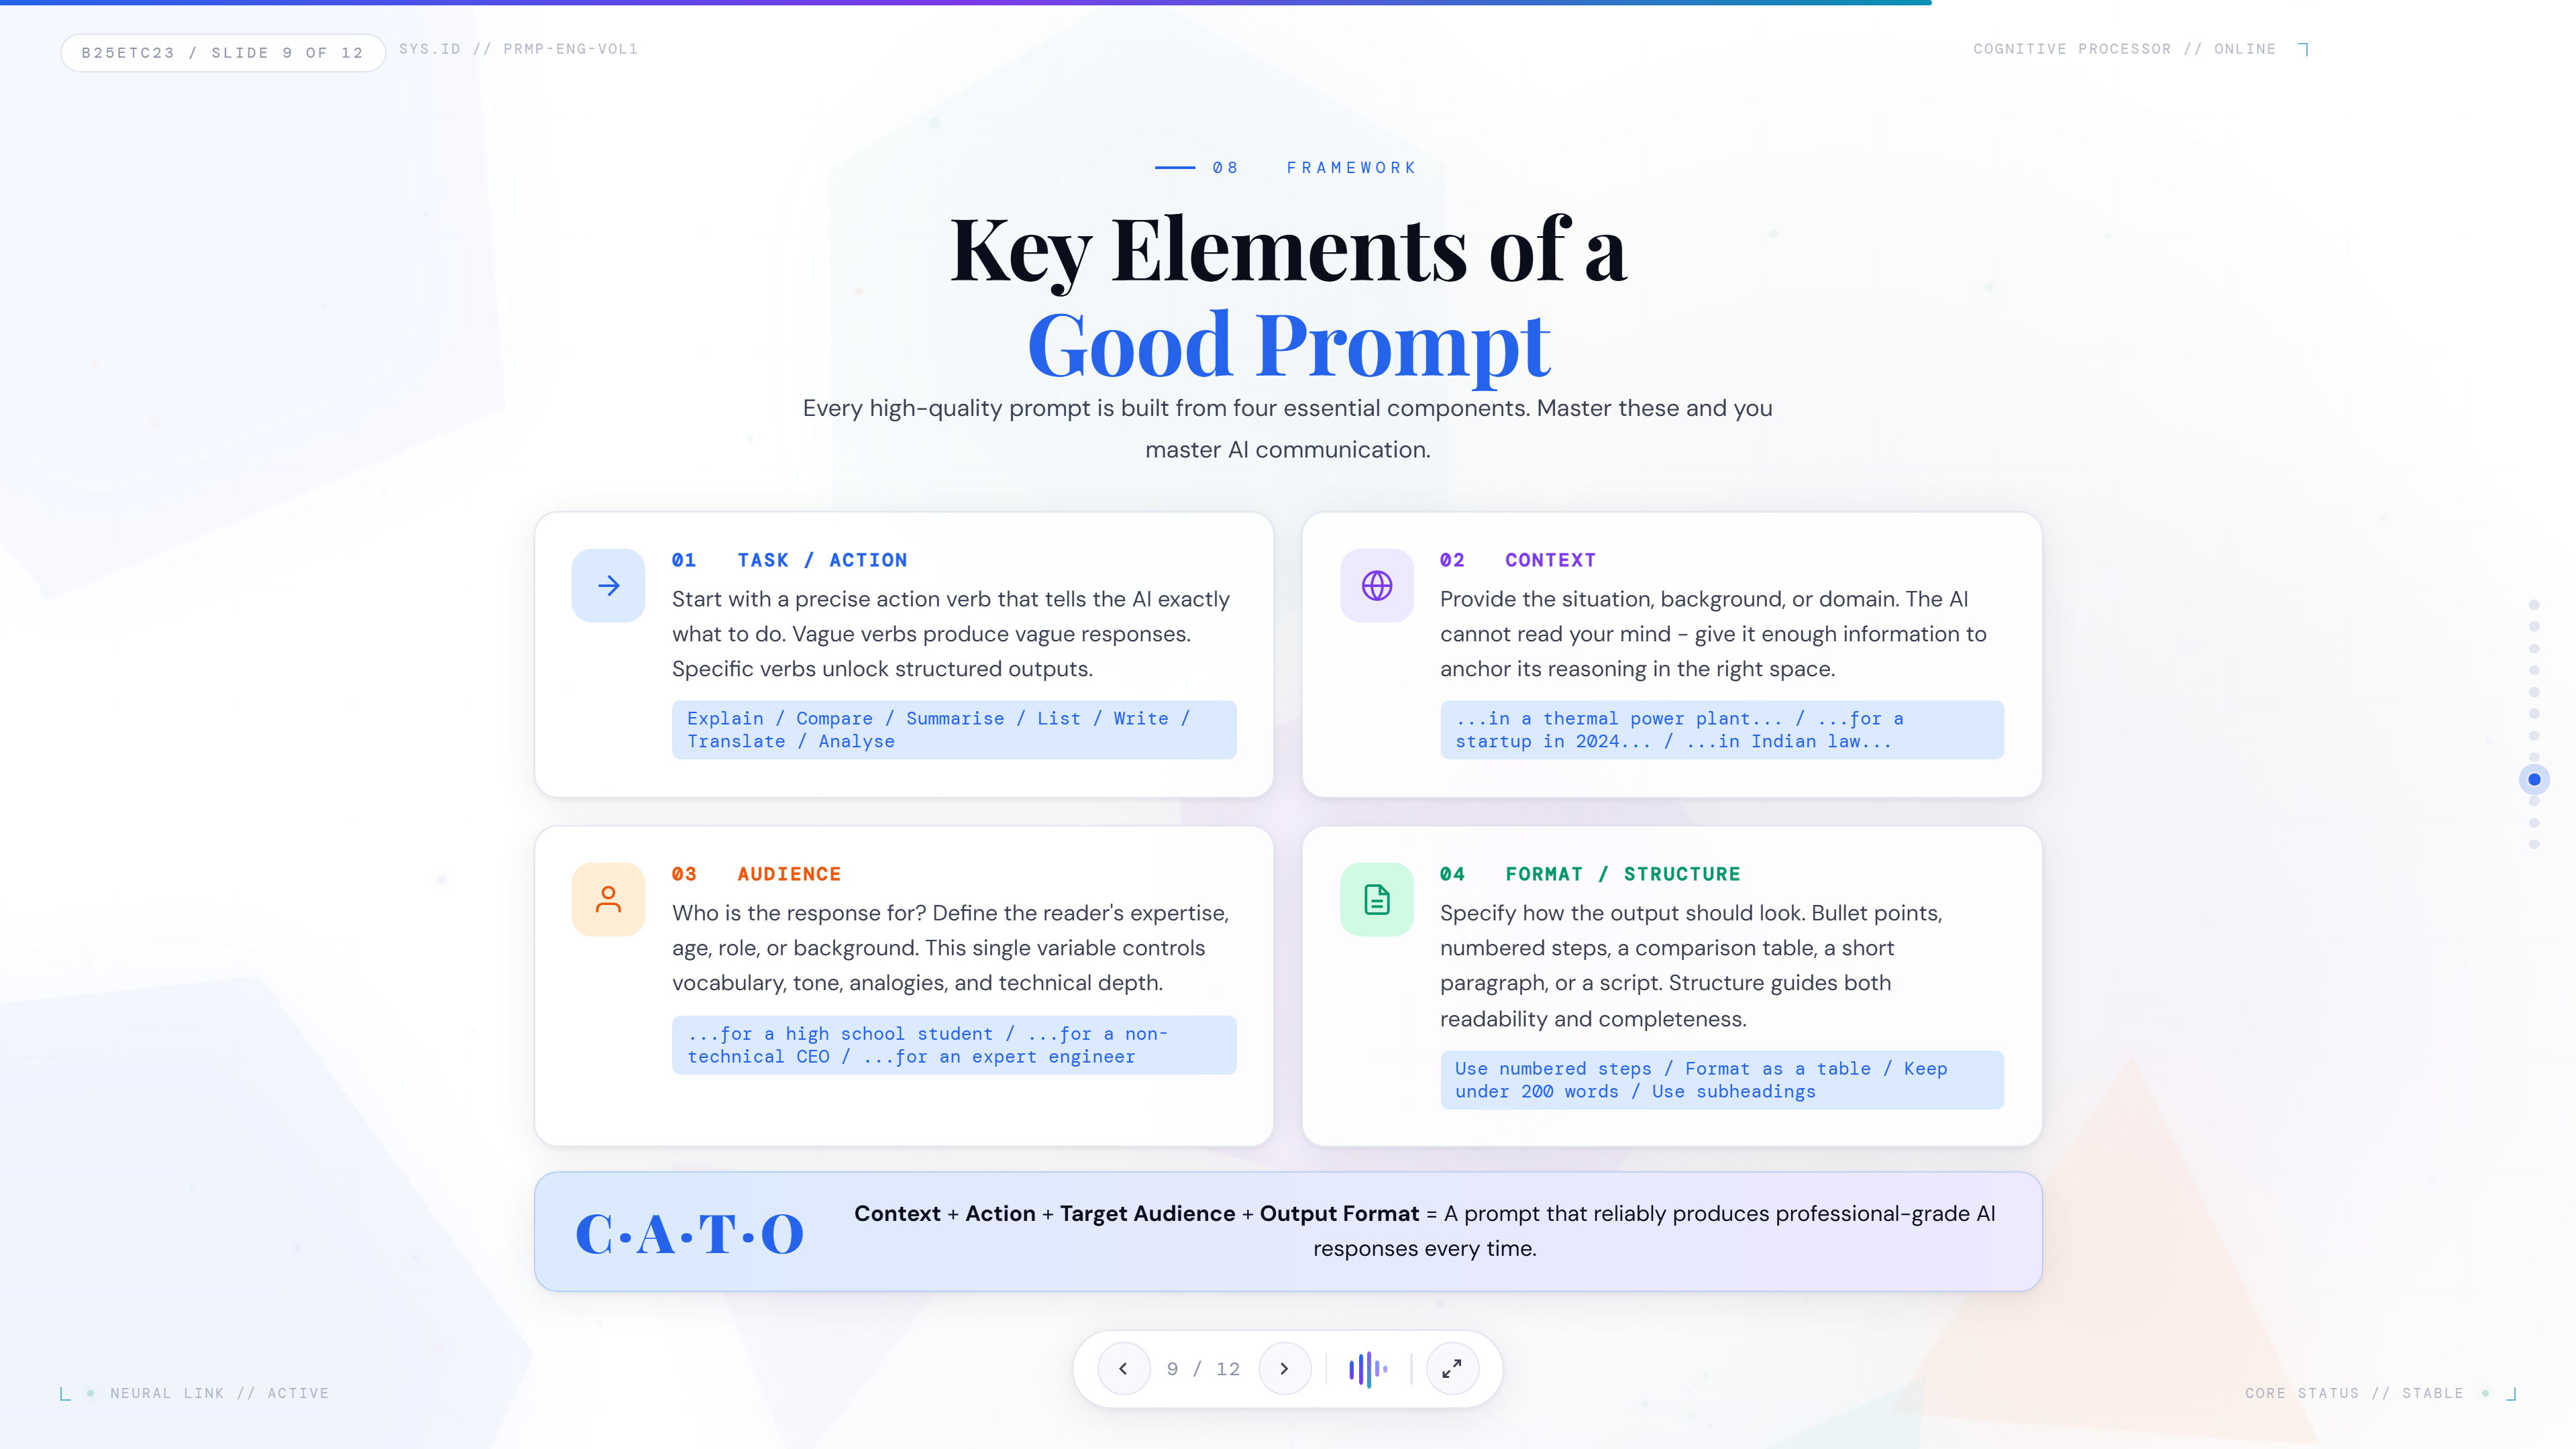
\includegraphics[width=0.92\textwidth]{slide_09.png}
  \caption{Slide 9: The CATO formula for effective prompts}
\end{figure}

From the experiment, a simple four-part framework was identified -- the \textbf{CATO formula}:

\begin{itemize}
  \item \textbf{C -- Context:} Provide the situation or background. The AI cannot read your mind. Example: \emph{``...in a thermal power plant...''}
  \item \textbf{A -- Action:} Start with a precise action verb. Explain, Compare, Summarise, List, Write, Analyse. Vague verbs produce vague results.
  \item \textbf{T -- Target Audience:} Define the reader's expertise, age, or role. This single variable controls vocabulary, tone, analogies, and depth. Example: \emph{``...for a high school student.''}
  \item \textbf{O -- Output Format:} Tell the AI how the response should look. Bullet points, numbered steps, a table, under 200 words.
\end{itemize}

\vspace{0.3cm}
\noindent\textbf{Context + Action + Target Audience + Output Format = Professional-grade AI response every time.}

Most people skip three of these four elements -- and that is why they get mediocre results.

\newpage

% ── Slide 10 ──
\subsection*{Slide 10 -- Tips and Best Practices}
\label{sec:s10}

\begin{figure}[H]
  \centering
  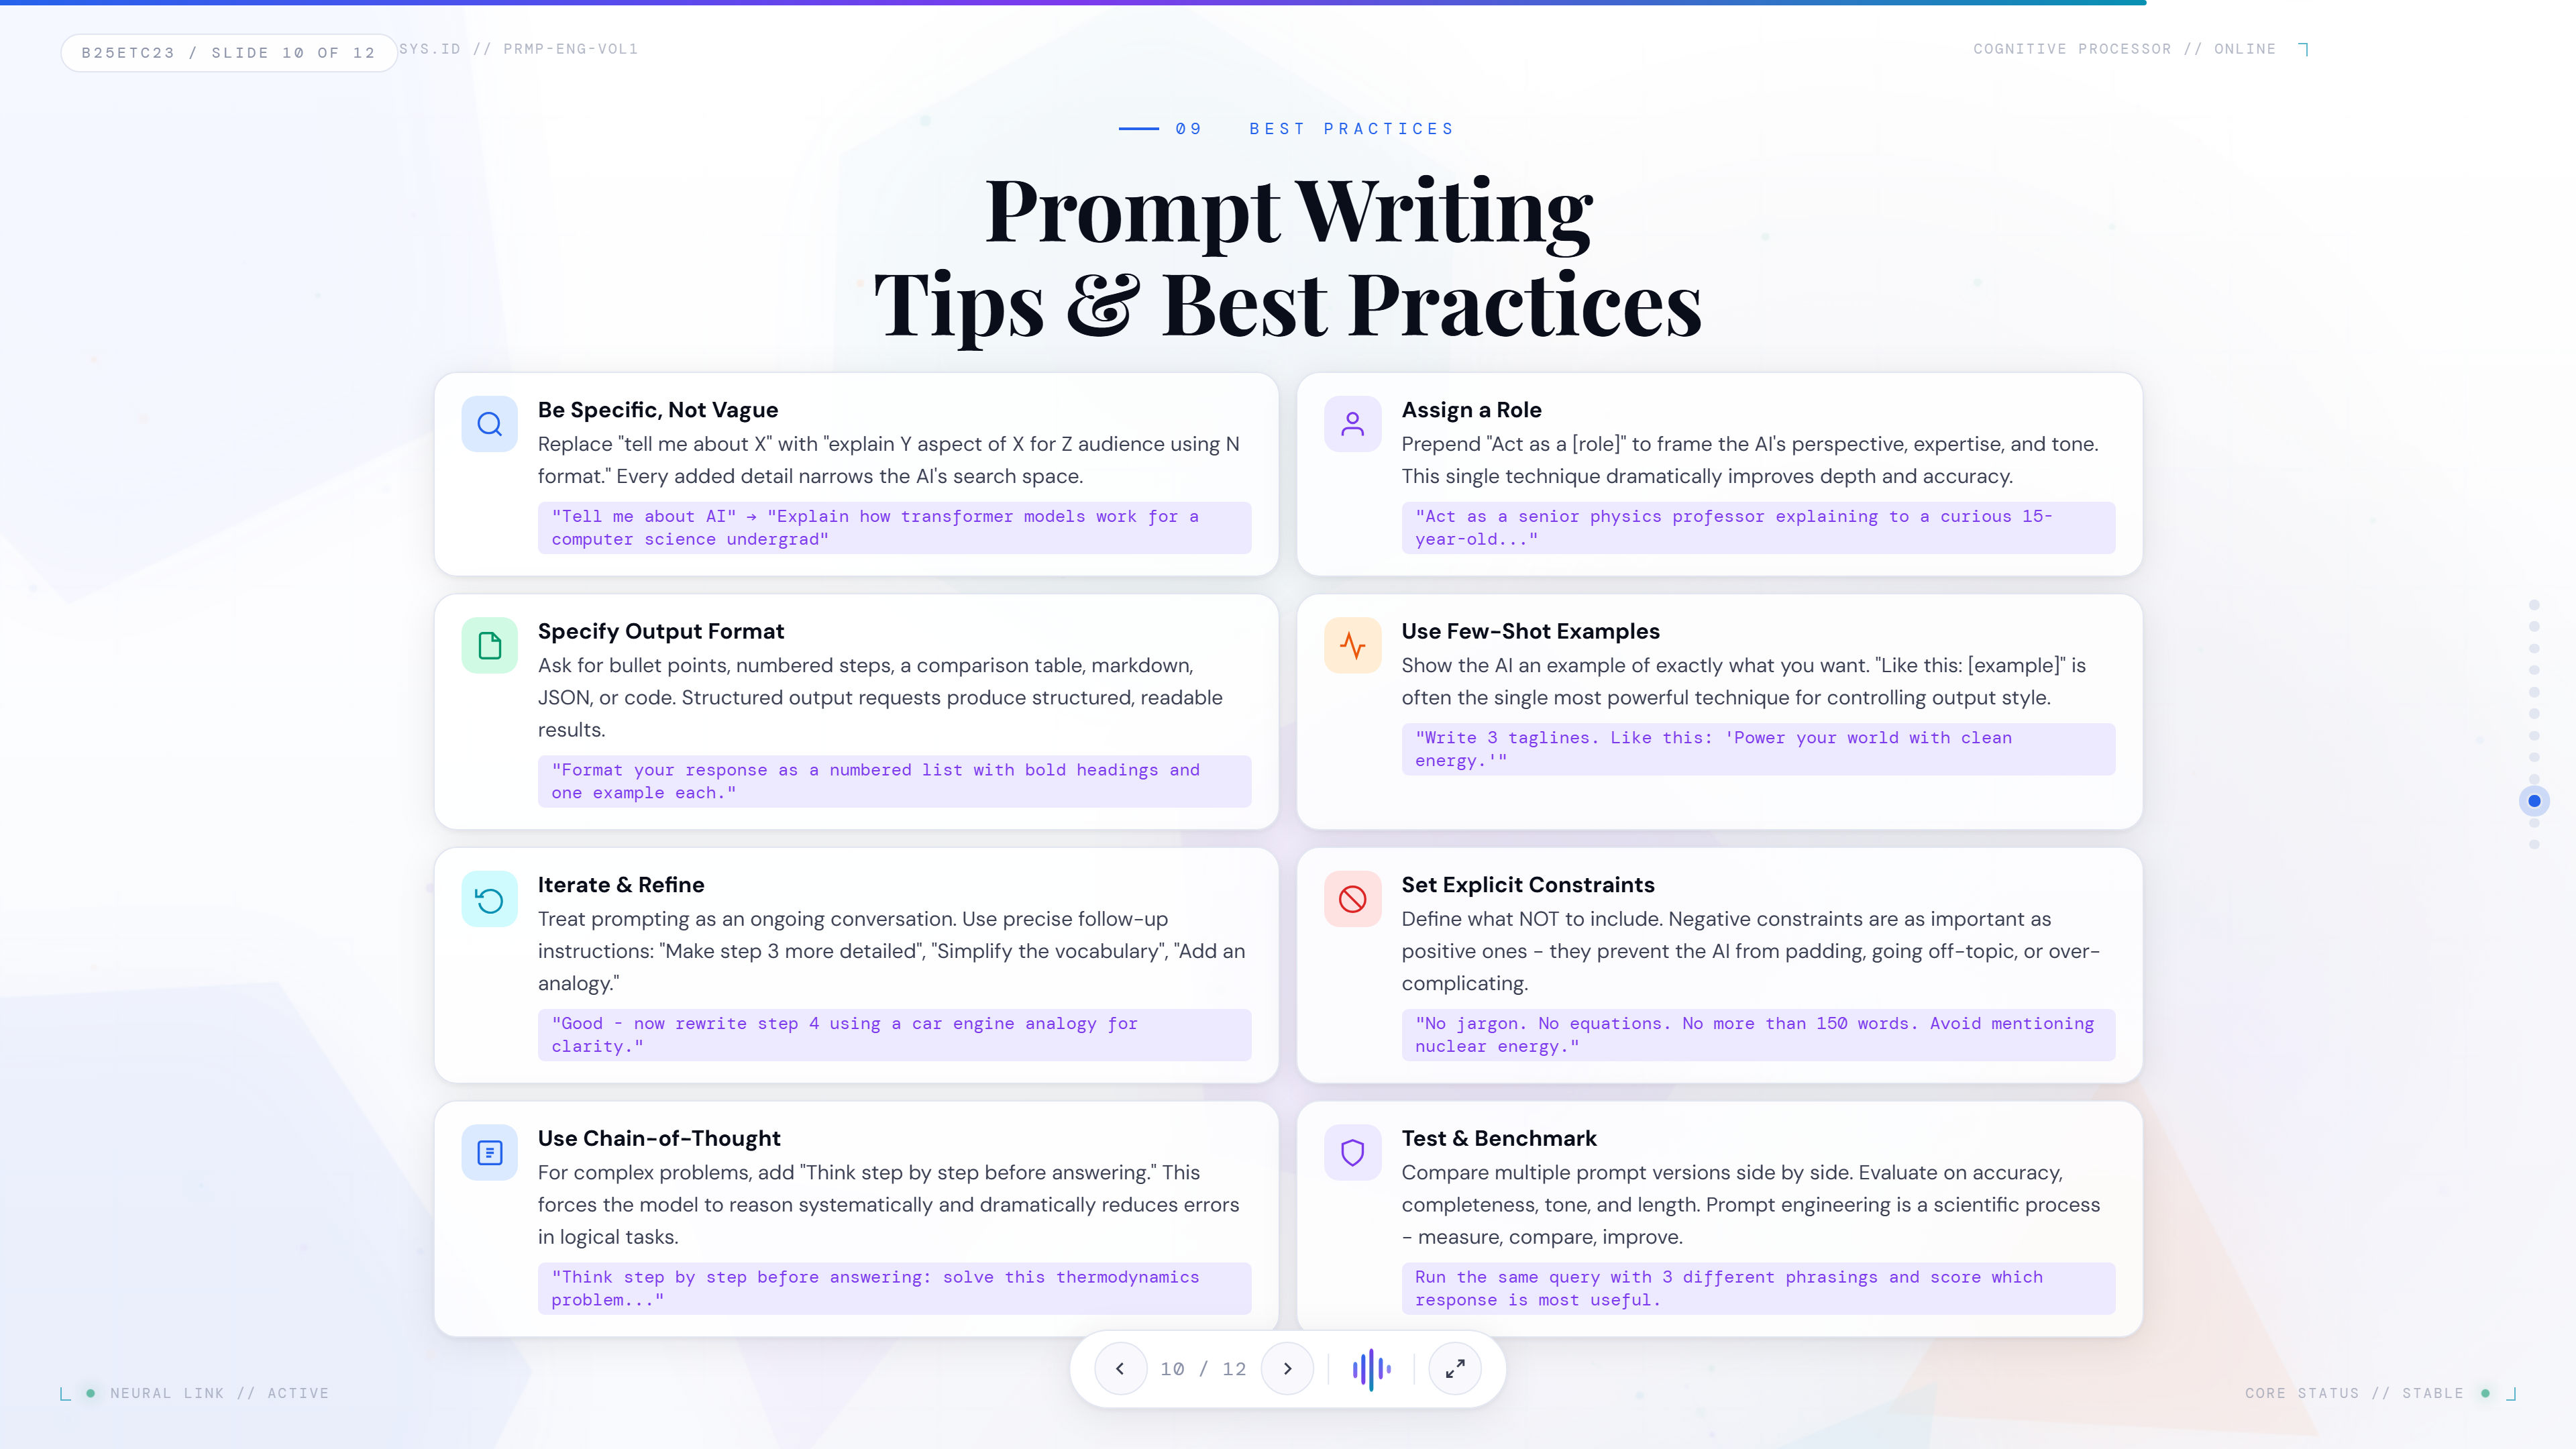
\includegraphics[width=0.92\textwidth]{slide_10.png}
  \caption{Slide 10: Eight practical prompt writing tips}
\end{figure}

This slide presents eight best practices for writing better prompts:

\begin{enumerate}
  \item \textbf{Be Specific, Not Vague} -- Replace ``tell me about X'' with a detailed instruction specifying aspect, audience, and format.
  \item \textbf{Assign a Role} -- Start with ``Act as a [role]'' to frame the AI's expertise and tone.
  \item \textbf{Specify Output Format} -- Ask for bullet points, numbered steps, a table, or even JSON.
  \item \textbf{Use Few-Shot Examples} -- Show the AI exactly what you want by providing examples.
  \item \textbf{Iterate and Refine} -- Treat it as a conversation; improve based on initial responses.
  \item \textbf{Set Explicit Constraints} -- Define what NOT to include. ``No jargon, no equations, no more than 150 words.''
  \item \textbf{Use Chain-of-Thought} -- For complex problems, add ``Think step by step before answering.''
  \item \textbf{Test and Benchmark} -- Run the same question with three different phrasings and compare results.
\end{enumerate}

\newpage

% ── Slide 11 ──
\subsection*{Slide 11 -- Real-World Applications}
\label{sec:s11}

\begin{figure}[H]
  \centering
  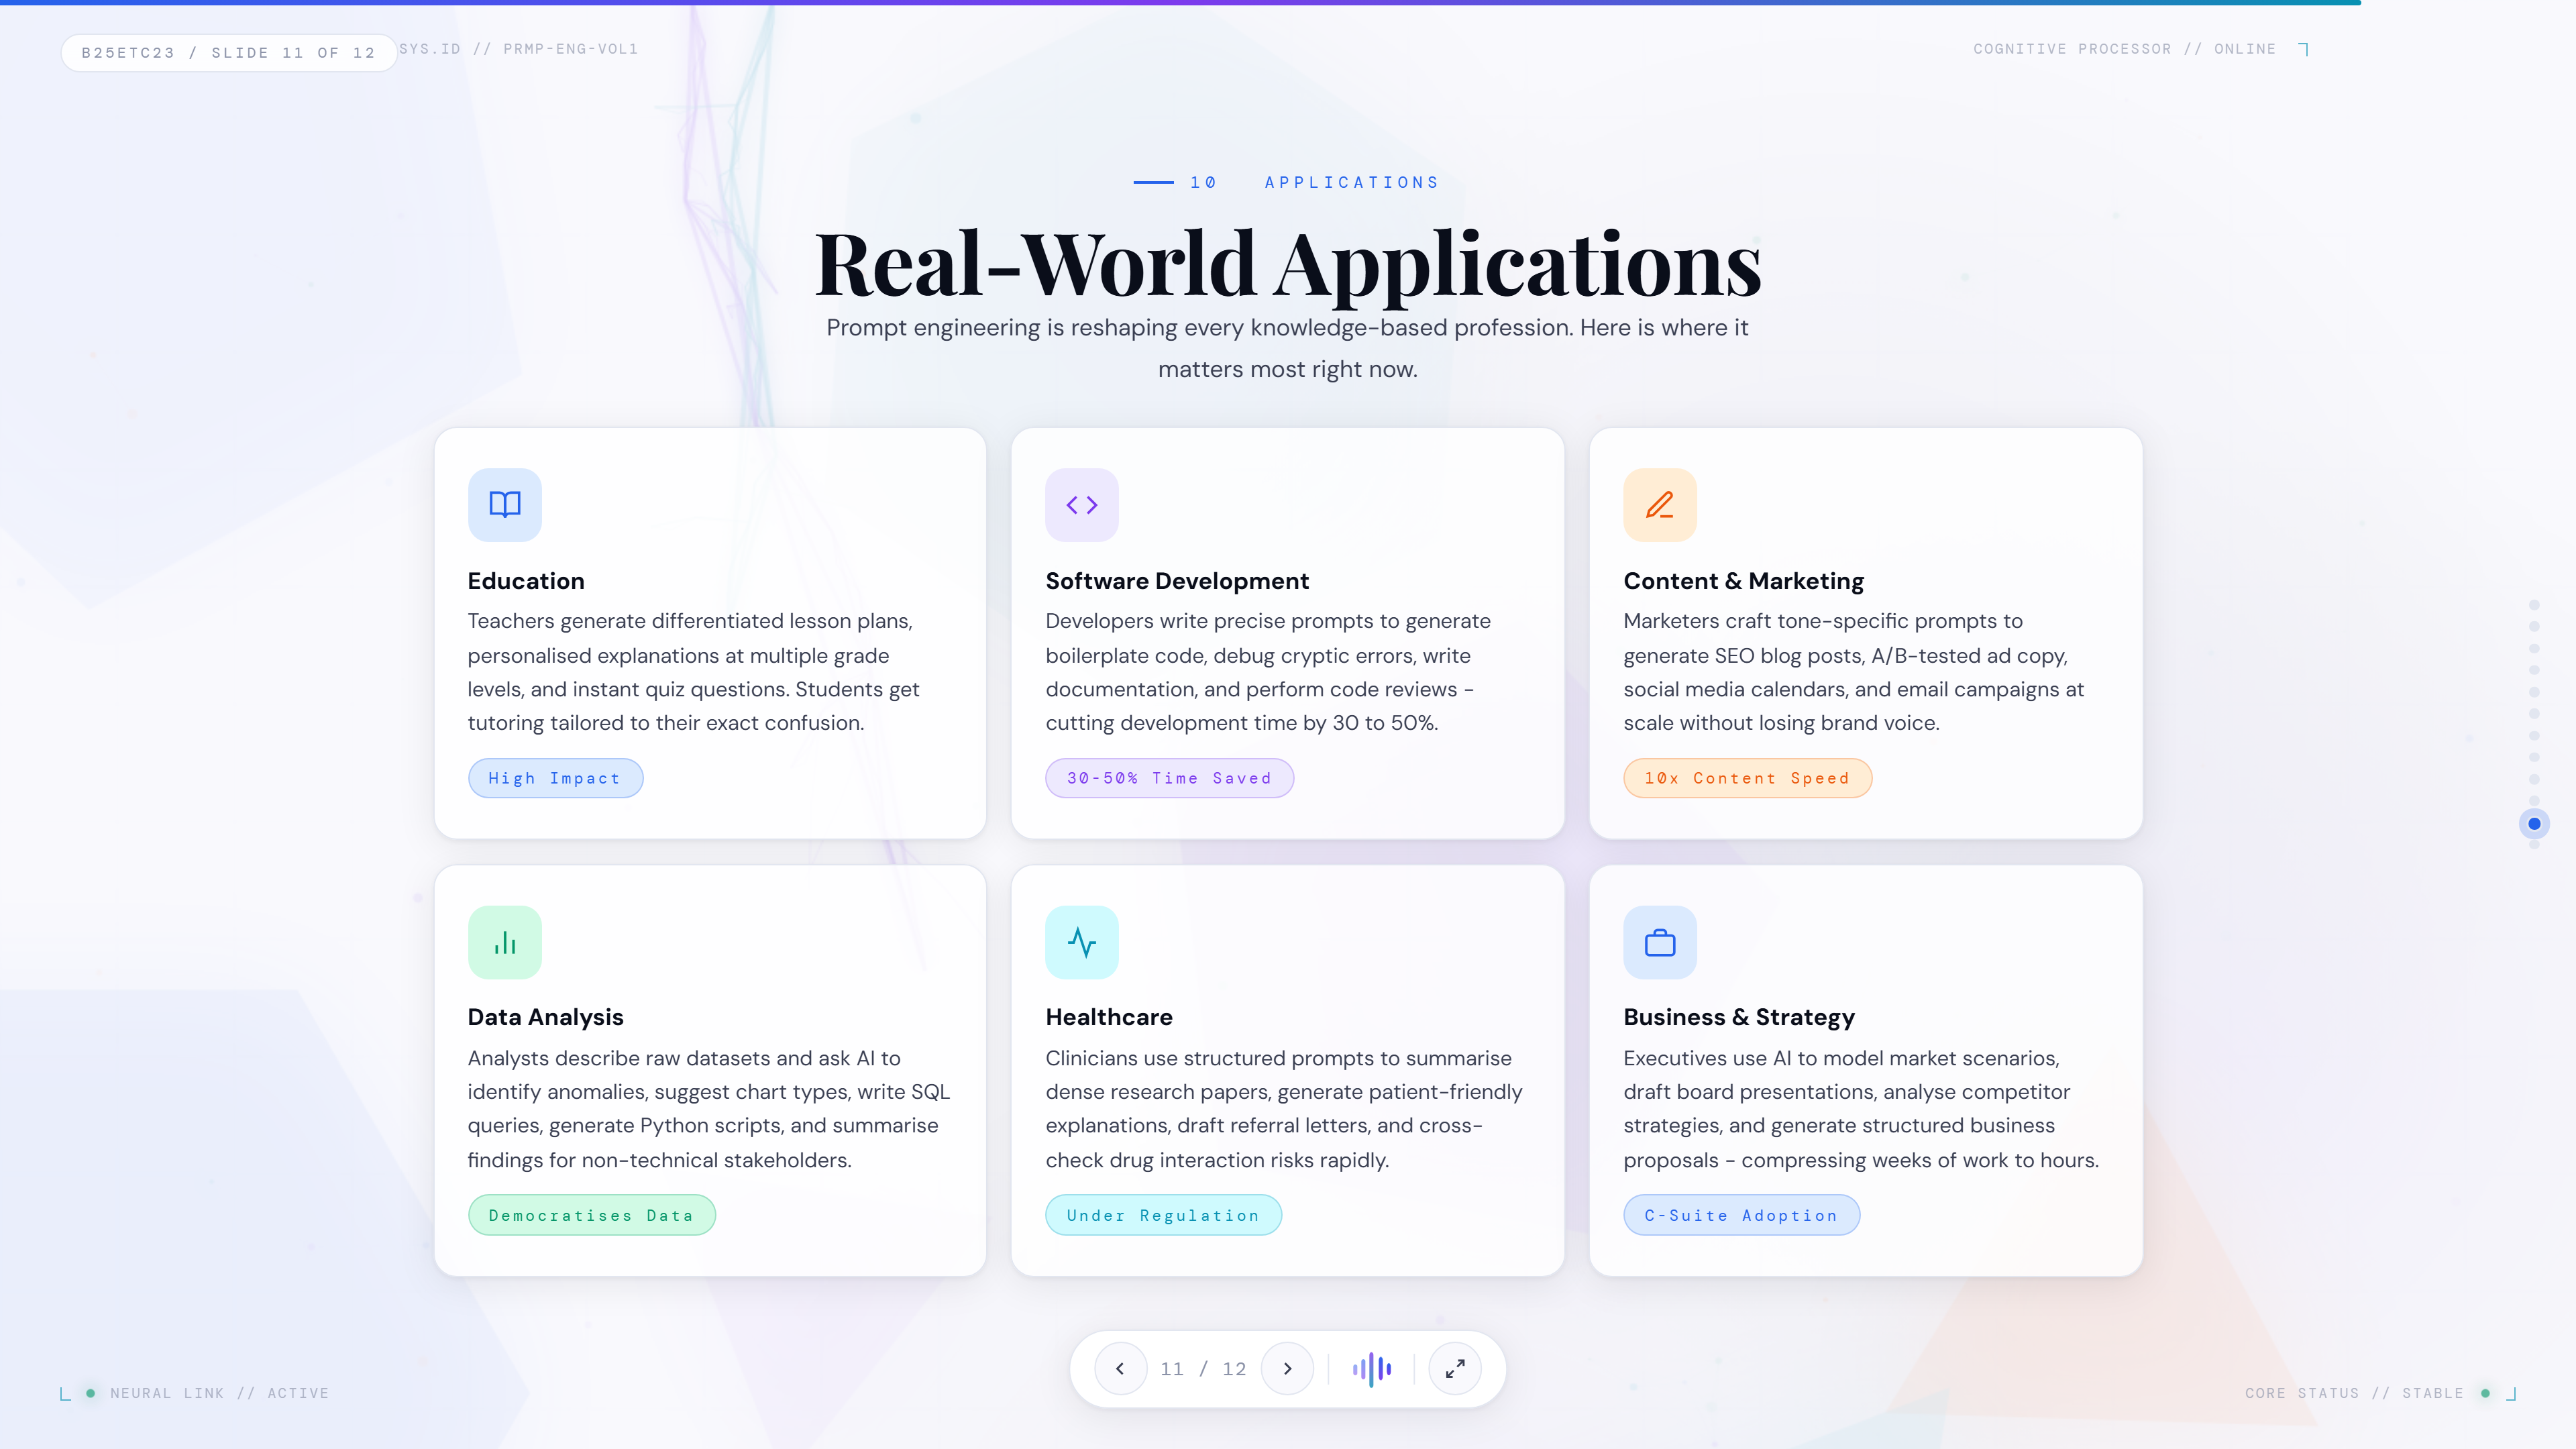
\includegraphics[width=0.92\textwidth]{slide_11.png}
  \caption{Slide 11: Prompt engineering applications across industries}
\end{figure}

This slide demonstrates that prompt engineering is already transforming real professions:

\begin{itemize}
  \item \textbf{Education} -- Teachers generate personalised lesson plans and quiz questions instantly. Students get tutoring tailored to where they are stuck.
  \item \textbf{Software Development} -- Developers use precise prompts to generate code, debug errors, and write documentation, cutting development time by 30 to 50 percent.
  \item \textbf{Content and Marketing} -- Marketers generate SEO articles, ad copy, and social media campaigns at scale without losing brand voice.
  \item \textbf{Data Analysis} -- Analysts prompt AI to write SQL queries, generate Python scripts, and summarise findings for non-technical managers.
  \item \textbf{Healthcare} -- Clinicians summarise research papers, generate patient-friendly explanations, and draft referral letters using structured prompts.
  \item \textbf{Business and Strategy} -- Executives model market scenarios, generate board presentations, and analyse competitors, compressing weeks of work into hours.
\end{itemize}

The common thread: \textbf{the people getting the most value from AI are the ones who know how to write a good prompt.}

\newpage

% ── Slide 12 ──
\subsection*{Slide 12 -- Conclusion}
\label{sec:s12}

\begin{figure}[H]
  \centering
  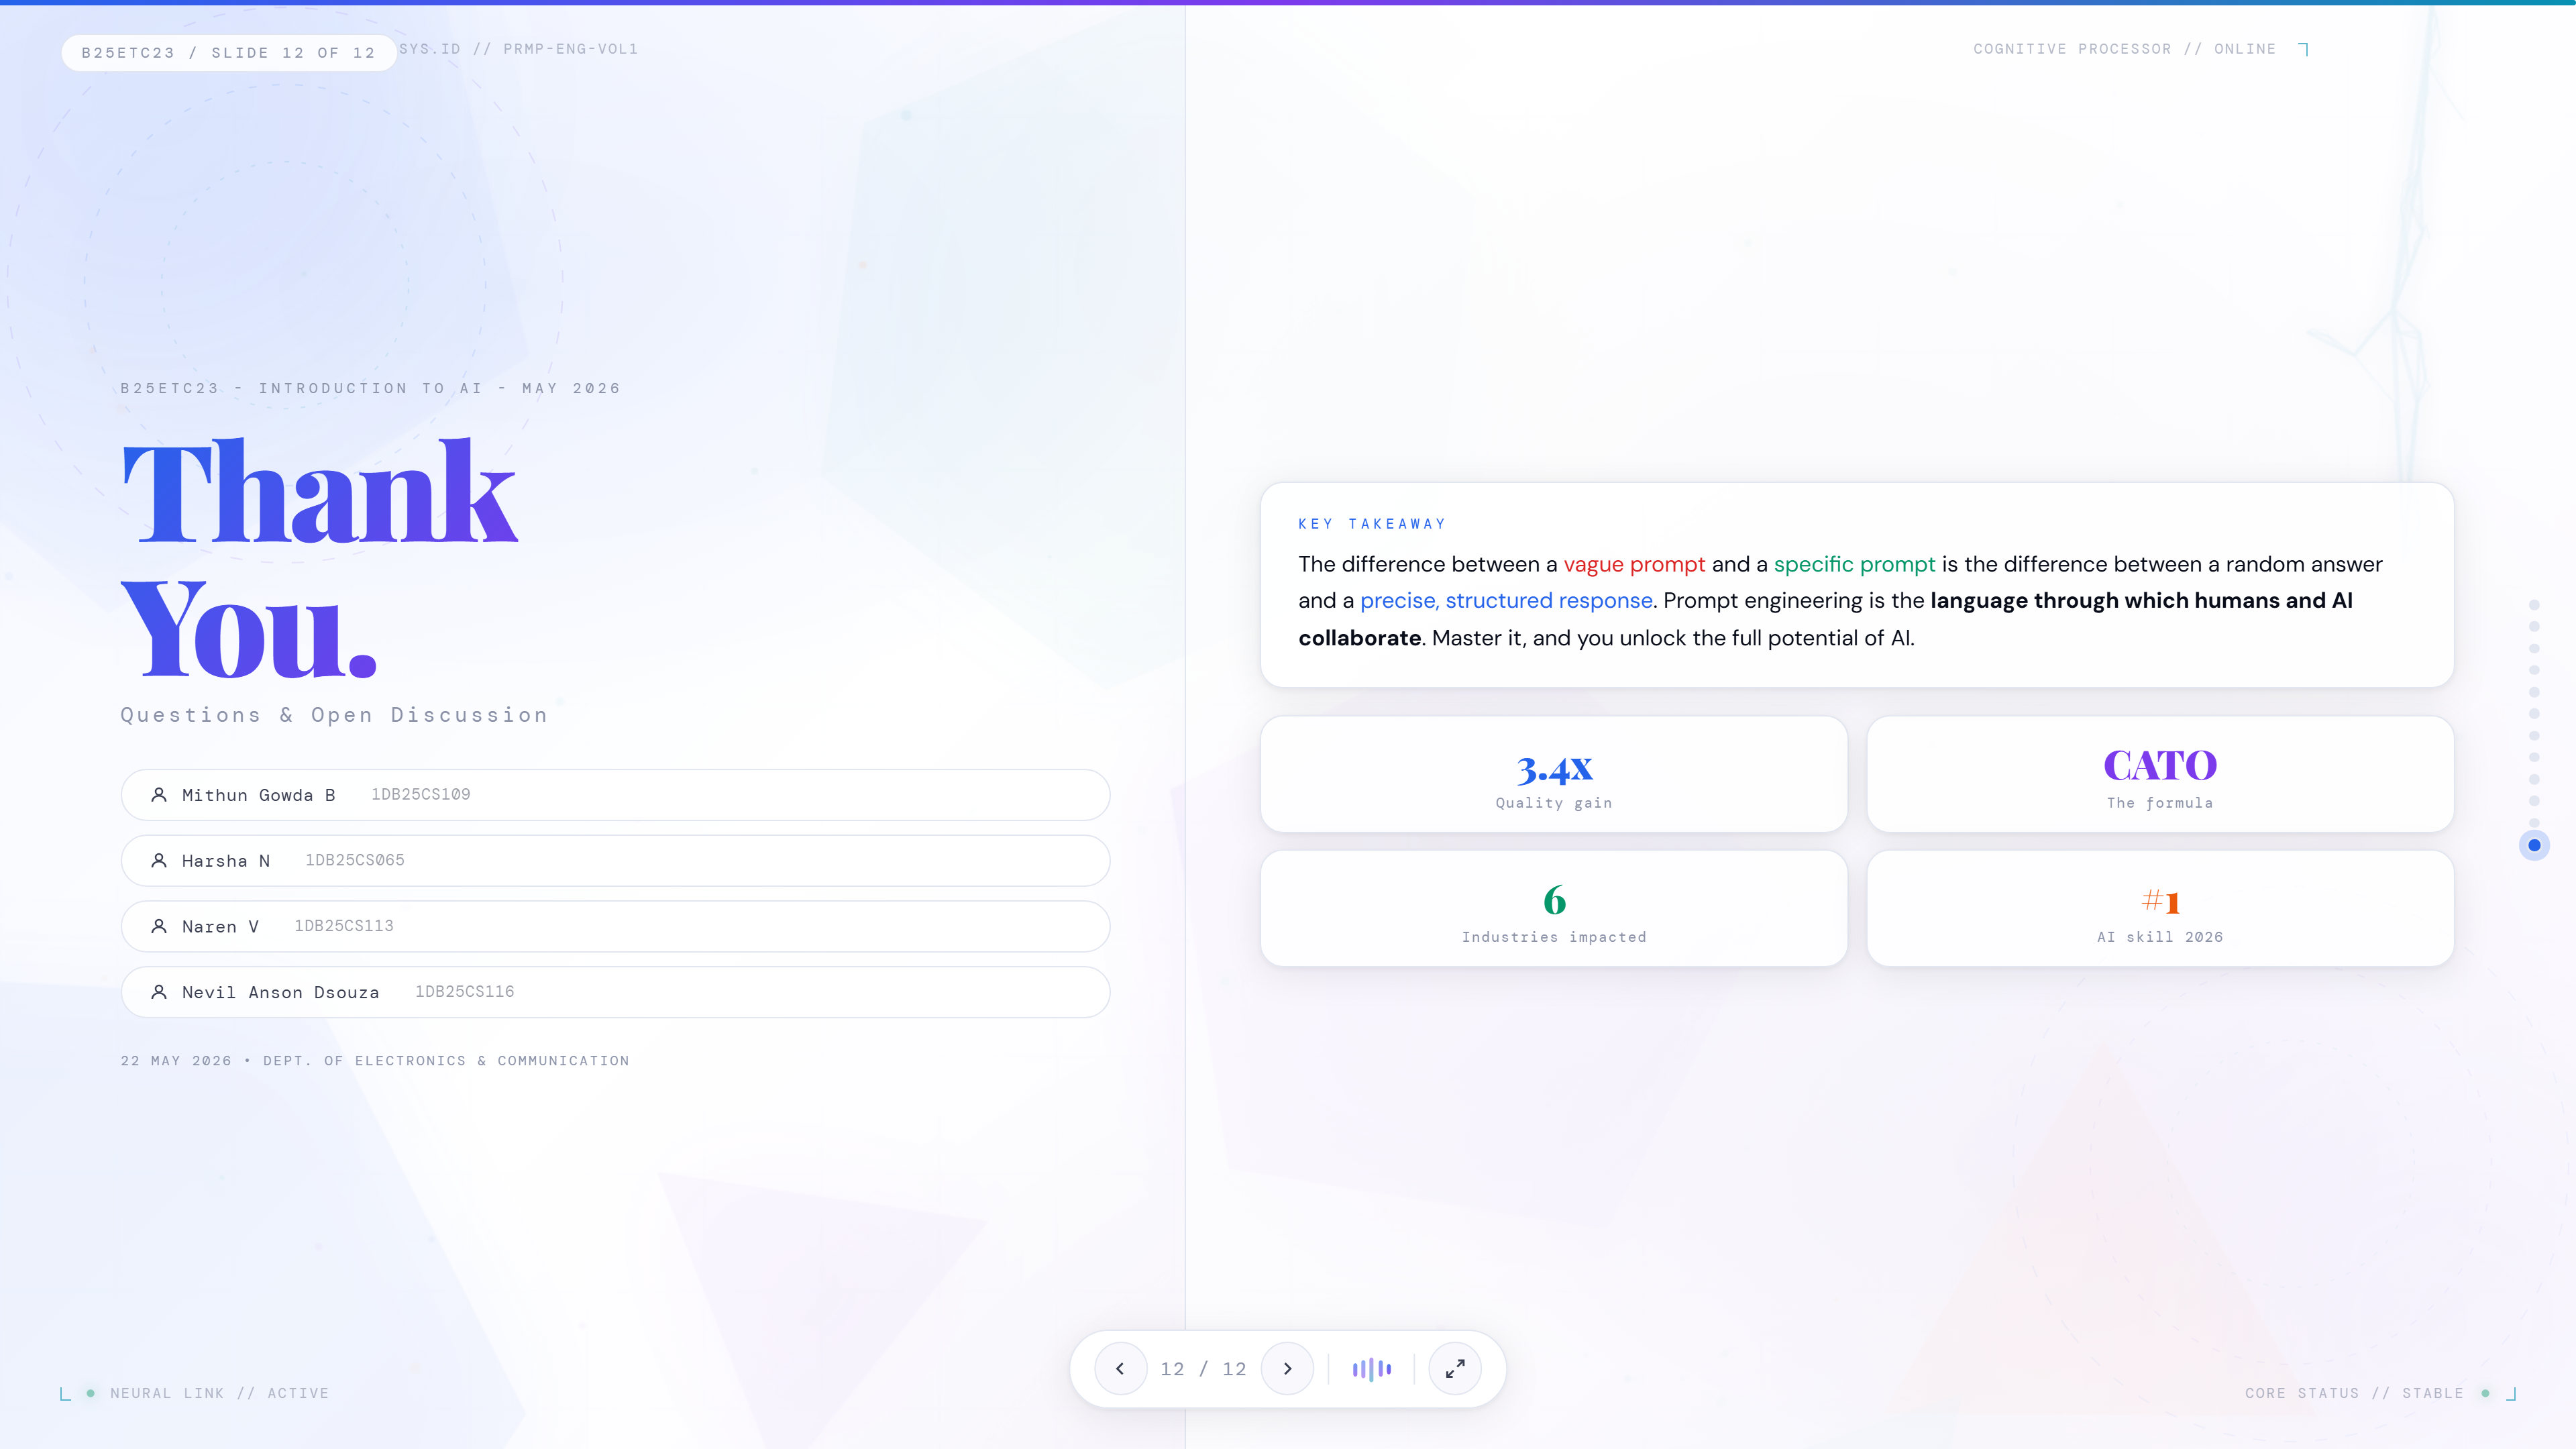
\includegraphics[width=0.92\textwidth]{slide_12.png}
  \caption{Slide 12: Conclusion and key takeaway}
\end{figure}

The concluding slide ties everything together. The core question -- does the way you phrase a question to an AI matter? -- has been answered conclusively.

The vague prompt \emph{``Tell me about electricity''} produced a generic, unstructured, unusable response. The specific prompt produced a structured, step-by-step, audience-appropriate explanation ready to use directly in an assignment.

\textbf{Same AI. Same topic. 3.4x better result -- from the prompt alone.}

The key takeaway: \emph{prompt engineering is the language through which humans and AI collaborate.} It is not a technical skill that only programmers need. It is a communication skill -- and it is already one of the most valuable skills in any knowledge-based job.

The CATO formula -- Context, Action, Target Audience, Output Format -- is your starting point. Use it every time you open ChatGPT or any other AI tool.

\vspace{1cm}
\begin{center}
\textit{Thank you for listening. We are happy to take any questions.}
\end{center}

\end{document}
